% -*- mode:flyspell; mode:latex -*-
% \documentclass[a4paper,twoside,11pt]{book}
\documentclass[12pt]{article}

\addtolength{\oddsidemargin} {-0.885in}
\addtolength{\textwidth}{1.75in}
\addtolength{\evensidemargin}{-0.8in}

\usepackage[latin1]{inputenc}
\usepackage[T1]{fontenc}
\usepackage[english]{babel}
\usepackage{float}
\usepackage{graphicx}
\usepackage{ulem}


\usepackage{tikz}
\usepackage{[caption}
\usetikzlibrary{arrows}
\usetikzlibrary{decorations.markings}
\usetikzlibrary{decorations.pathmorphing}
% \usepackage[absolute,overlay]{textpos}
% \usepackage{onimage}

\usepackage{times}

% \usepackage{subfigure}
% \usepackage{scalefnt}
% 
% \renewcommand\thesubfigure{\arabic{subfigure}}

\usepackage{amsmath}
\usepackage{hyperref}
\usepackage{hhline}
\usepackage{subfig}
\usepackage{color}
\usepackage[all]{hypcap}

% \usepackage[normalem]{ulem}  % for striking out
% \usepackage{fancyhdr}
% \pagestyle{fancy}
% \fancyhead[C]{}
% \fancyhead[L] {\it{Mu2e-doc-29670-v1.0} }
%%%%%%%%%%%%%%%%%%%%%%%%%%%%%%%%%%%%%%%%%%%%%%%%%%%%%%%%%%%%%%%%%%%%%%%%%%%%%%
% use natbib - biblatex not available on Mu2e interactive nodes
%%%%%%%%%%%%%%%%%%%%%%%%%%%%%%%%%%%%%%%%%%%%%%%%%%%%%%%%%%%%%%%%%%%%%%%%%%%%%%
\usepackage[square,sort,comma,numbers]{natbib}

% location of the .bib files: env var BIBINPUTS (~/library/bibliography)

% \usepackage[backend=biber, style=numeric-comp, sorting=ynt] {biblatex}
% \addbibresource{clfv.bib}

% \addbibresource{stntuple.bib}
% \addbibresource{mu2e_web.bib}
% \addbibresource{radiative_pion_capture.bib}

\graphicspath{{figures/}}
%%%%%%%%%%%%%%%%%%%%%%%%%%%%%%%%%%%%%%%%%%%%%%%%%%%%%%%%%%%%%%%%%%%%%%%%%%%%%%
% for portability, make sure all commands are included locally
%%%%%%%%%%%%%%%%%%%%%%%%%%%%%%%%%%%%%%%%%%%%%%%%%%%%%%%%%%%%%%%%%%%%%%%%%%%%%%
%\include{commands}
\newcommand {\kmax}            {\mbox{$k_{\rm max}$}}
\newcommand {\mumemconv}[1][A] {\mbox{$\mu^- \textrm{#1} \rightarrow e^- \textrm{#1}$}}

% Define a relay to have 2 default arguments instead of limit of 1
\newcommand {\mumepconv}[1][A] {%
  \def\ArgI{{#1}}%store the first argument
  \mumepconvRelay
}
\newcommand \mumepconvRelay[1][A]  {\mbox{$\mu^- \textrm{\ArgI} \rightarrow e^+ \textrm{#1}$}}
\newcommand {\MuToEm}     {\mbox{$\mu^- \ra e^-$}}
\newcommand {\MuToEp}     {\mbox{$\mu^- \ra e^+$}}
\newcommand {\MuPToEp}    {\mbox{$\mu^+ \ra e^+$}}

\newcommand {\ra}        {\rightarrow}
\newcommand {\red}       {\color{red} }
\newcommand {\blue}      {\color{blue}}
\newcommand {\tandip}    {\mbox{$\tan \lambda$}}

\newcommand {\Pb}[1]     {\mbox{$\rm ^{#1}Pb$}}                 % isotopes of lead
\newcommand {\Au}[1]     {\mbox{$\rm ^{#1}Au$}}                 % isotopes of gold
\newcommand {\Ir}[1]     {\mbox{$\rm ^{#1}Ir$}}                 % isotopes of iridium

\newcommand {\strike}[1] {{\blue \sout{#1}}}
%%%%%%%%%%%%%%%%%%%%%%%%%%%%%%%%%%%%%%%%%%%%%%%%%%%%%%%%%%%%%%%%%%%%%%%%%%%%%%
\begin{document}

\begin{titlepage}
  \begin{flushright}
    \bf {MU2E/PHYSICS/36375} \\
    version 1.00
    \today
 \end{flushright}

  \vspace{1cm}
  
  \begin{center}
    {\Large \bf Mu2e 2020 sensitivity update. \\
      \vspace {0,2in} 
      2. Reconstruction} 
    
    \vspace{1cm}
    
    S. Di Falco (INFN Pisa), S. Huang (Purdue Univ.,
    M. MacKenzie (Northwestern Univ.),
    P. Murat(FNAL)
    
    % \footnote{\texttt{Fermilab; e-mail: murat@fnal.gov}}
    \vspace{0.3cm}
    
    \vspace{0.8cm}                           
  \end{center}

  \begin{abstract}
    This note documents changes made to the Mu2e reconstruction software
    used for 2020 sensitivity update (SU2020).
  \end{abstract}

\end{titlepage}
% \frontmatter
% \chapter*{Abstract}
%
% \addcontentsline{toc}{chapter}{Abstract}
%
% \mainmatter
%
{\tableofcontents}

%%%%%%%%%%%%%%%%%%%%%%%%%%%%%%%%%%%%%%%%%%%%%%%%%%%%%%%%%%%%%%%%%%%%%%%%%%%%%%%
%\chapter{Calibration}
%%%%%%%%%%%%%%%%%%%%%%%%%%%%%%%%%%%%%%%%%%%%%%%%%%%%%%%%%%%%%%%%%%%%%%%%%%%%%%%
% \input{input_data}

%%%%%%%%%%%%%%%%%%%%%%%%%%%%%%%%%%%%%%%%%%%%%%%%%%%%%%%%%%%%%%%%%%%%%%%%%%%%%%%

\newpage
\section { Introduction}
All datasets referred to in this note are described in \cite{MU2E_36372_SU2020_DATASETS}.

% -*- mode:latex; mode:flyspell -*-
%%%%%%%%%%%%%%%%%%%%%%%%%%%%%%%%%%%%%%%%%%%%%%%%%%%%%%%%%%%%%%%%%%%%%%%%%%%%%%
\section{Correcting {\blue the} relative tracker-calorimeter timing offset}

In an event \strike{which} {\blue that} has a calorimeter cluster \strike{matching} {\blue matched}
to a reconstructed track, the
cluster is included in\strike{to} the track fit as an additional hit. 
\strike{The algorithm reconstructing 
straw hits in the tracker and the algorithm reconstructing the waveform timing in the calorimeter
could add different timing offsets to the reconstructed hist and clusters correspondingly.
Those offsets need to be calibrated out.}
{\blue The straw hit reconstruction algorithm in the tracker and the waveform reconstruction 
algorithm
in the calorimeter can add different timing offsets to the reconstructed straw hits and 
calorimeter
clusters respectively; these timing offsets need to be calibrated out.}

\strike{A cluster is included into the track fit with the coordinate error $\sigma_{XY} = 15$ mm
and the timing error $\sigma_T = 0.5ns$.}

{\blue The cluster is included in the track fit with a coordinate error $\sigma_{XY} = 15$ mm
and a timing error $\sigma_T = 0.5$ ns.}
The distribution of the calorimeter cluster timing residuals for conversion electrons \strike{and}
{\blue using the} default Kalman fit 
configuration is shown in Figure \ref{fig:track_cluster_dt}.a. 
The distribution of cluster timing residuals 
is centered at about -1.17 ns and has a width of about 0.34 ns, \strike{indicating presence of
the systematic effect.} {\blue indicating a systematic timing offet.}

To study the \strike{effect} {\blue systematic offset} and avoid biasing the fit, the 
{\blue coordinate and timing} errors assigned to the 
cluster were increased to $10^6$ \strike{(ns or mm)} {\blue ns and $10^6$ mm respectively},
the corresponding distribution in timing residuals is shown in Figure 
\ref{fig:track_cluster_dt}.b. 
In this case, \strike{inclusion of} {\blue including} the cluster in\strike{to} the track fit
\strike{doesn't}
{\blue does not} bias the result of the fit and {\blue so} one can conclude 
that there is a systematic timing offset between the tracker and the calorimeter\strike{, 
which value is about 1.6 ns.} {\blue of about 1.6 ns.}
Figure \ref{fig:track_cluster_dt}.c corresponds to \strike{the} {\blue a} fit configuration with
the cluster time corrected by 1.6 ns, {\blue where, although the errors are large, the}
\strike{and still large errors, and one can see that the} applied correction zeroes the timing offset.

{\blue The d}\strike{D}istribution of timing residuals with the cluster time corrected by 
\strike{1.6ns} {\blue 1.6 ns} and {\blue using the} default 
{\blue coordinate and timing} errors (\strike{0.5ns and 15mm} {\blue 0.5 ns and 15 mm respectively}) 
assigned to the cluster shows a systematic shift of about \strike{0.5-0.6ns} {\blue 0.5-0.6 ns},
apparently introduced by the fitting procedure.
{\blue For now, we correct this additional cluster timing offset and use the default errors 
assigned to the calorimeter cluster in the Kalman fit.}

\strike{For now, we correct the cluster timing and use the default resolutions assigned to the calorimeter cluster 
in the Kalman fit.}

Correction of the the global track-to-calorimeter timing offset \strike{have} {\blue has (had?)} been introduced {\bf before} 
the tuning of the calorimeter timing resolution \strike{has} {\blue had} been completed. The global correction zeroing the offset
of the timing residuals was 1.86 ns, whereas after the tuning, the observed offset value is about 1.6 ns.
{\blue The r}\strike{R}esulting{\blue , un}\strike{non-}accounted for{\blue ,} systematic offset of about 0.25 ns is however about x2 smaller than the offset
introduced by the Kalman fitter. {\blue Not entirely clear what this paragraph is saying about the order of offsets
and what the 1.86 ns offset is/came from, perhaps re-wording?}

It is also worth noting that the width of the distribution of the calorimeter cluster timing residuals is
approximately 50\% of the error assigned to the cluster. The proportionality stays the same, about 50\%\strike{ level},  
when the timing error assigned to the cluster varies in the range [0.25 ns, 1 ns]. That is another indication
of a {\blue un}\strike{non-}compensated systematic effect related to the use of the calorimeter cluster in the Kalman fit.

\begin{figure}[h]
  \hspace{-0.8in}
  \begin{tikzpicture}
    \node[anchor=south west,inner sep=0] at (0,0.) {
      % \node[shift={(0 cm,0.cm)},inner sep=0,rotate={90}] at (0,0) {}
      % \makebox[\textwidth][c] {
      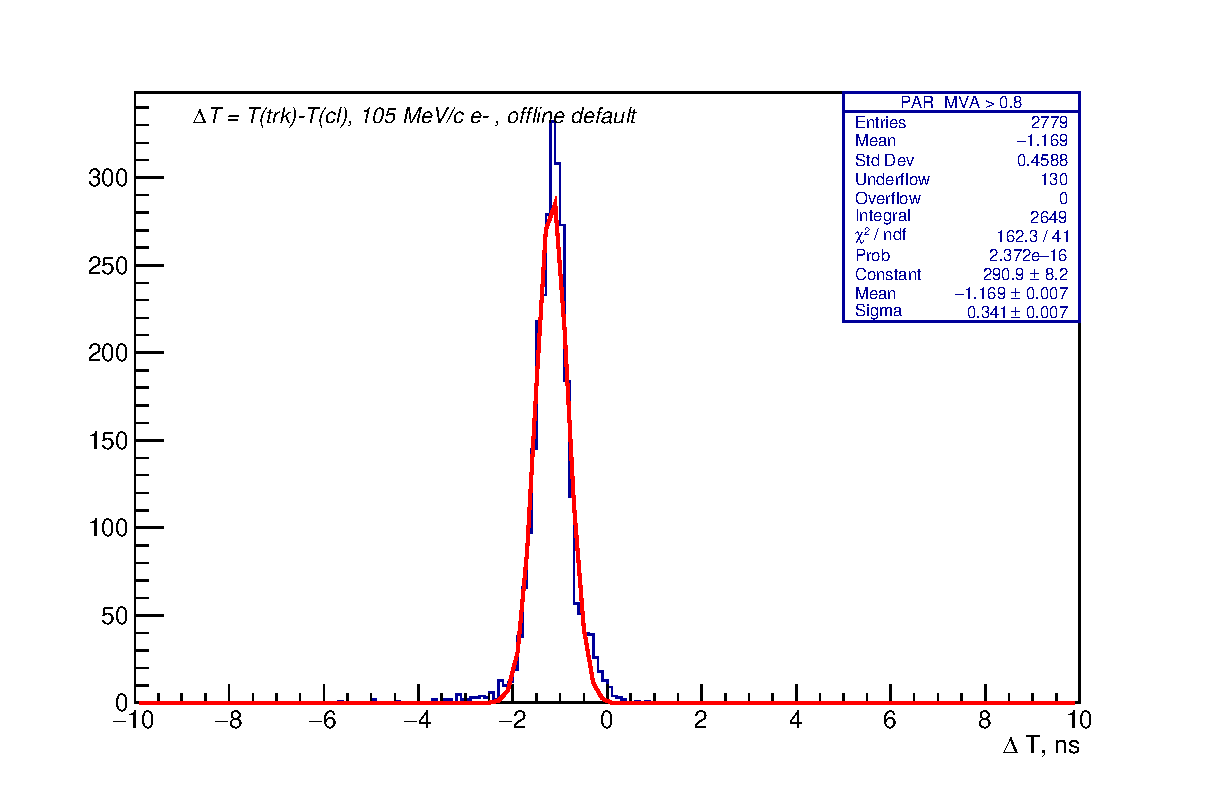
\includegraphics[width=0.64\textwidth]{figures/pdf/figure_00131_ele00s51b0_su2020_track_ana_trk_200_dt}
      % }
    };
    \node [text width=1cm, scale=0.8] at (3.,5) {(a)};
    \node[anchor=south west,inner sep=0] at (10.7,0.) {
      % \node[shift={(0 cm,0.cm)},inner sep=0,rotate={90}] at (0,0) {}
      % \makebox[\textwidth][c] {
      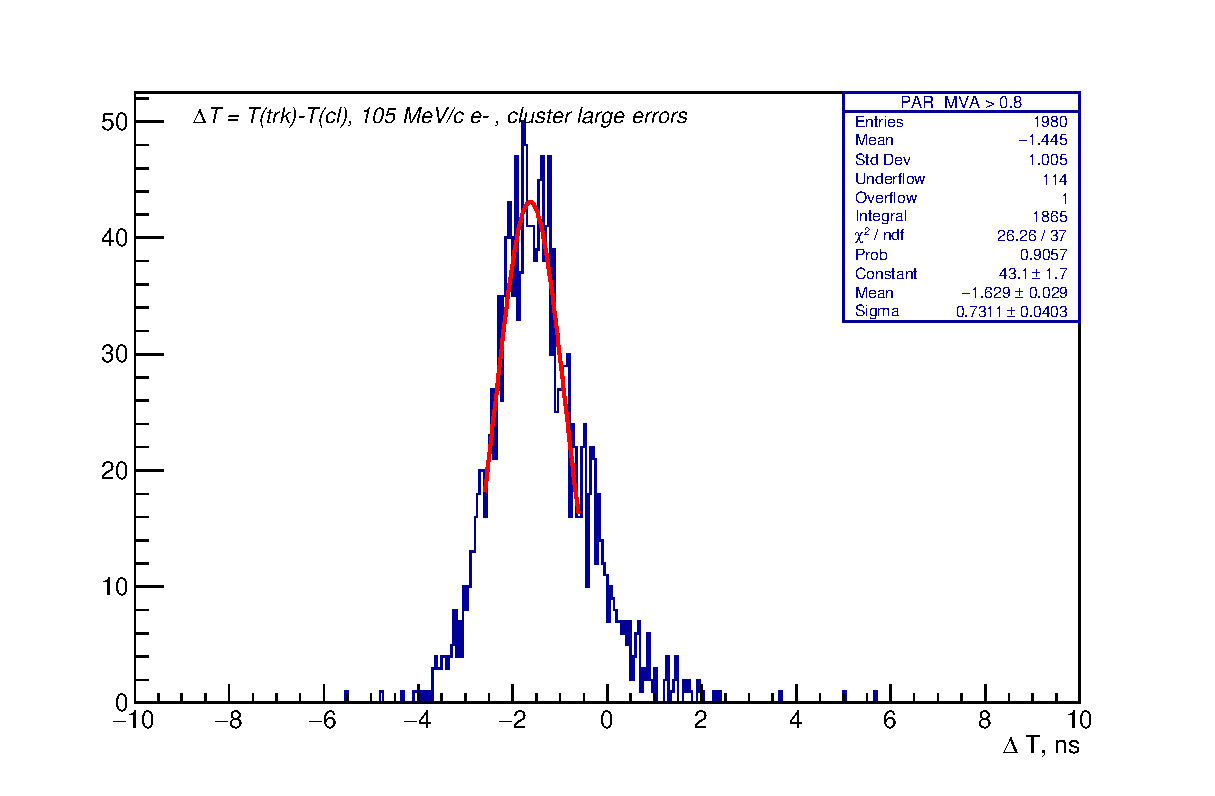
\includegraphics[width=0.64\textwidth]{figures/pdf/figure_00132_ele00s51b0_pid_emuana_trk_101_dt}
      % }
    };
    \node [text width=1cm, scale=0.8] at (13.7,5) {(b)};
    \node[anchor=south west,inner sep=0] at (0,-7.0) {
      % \node[shift={(0 cm,0.cm)},inner sep=0,rotate={90}] at (0,0) {}
      % \makebox[\textwidth][c] {
      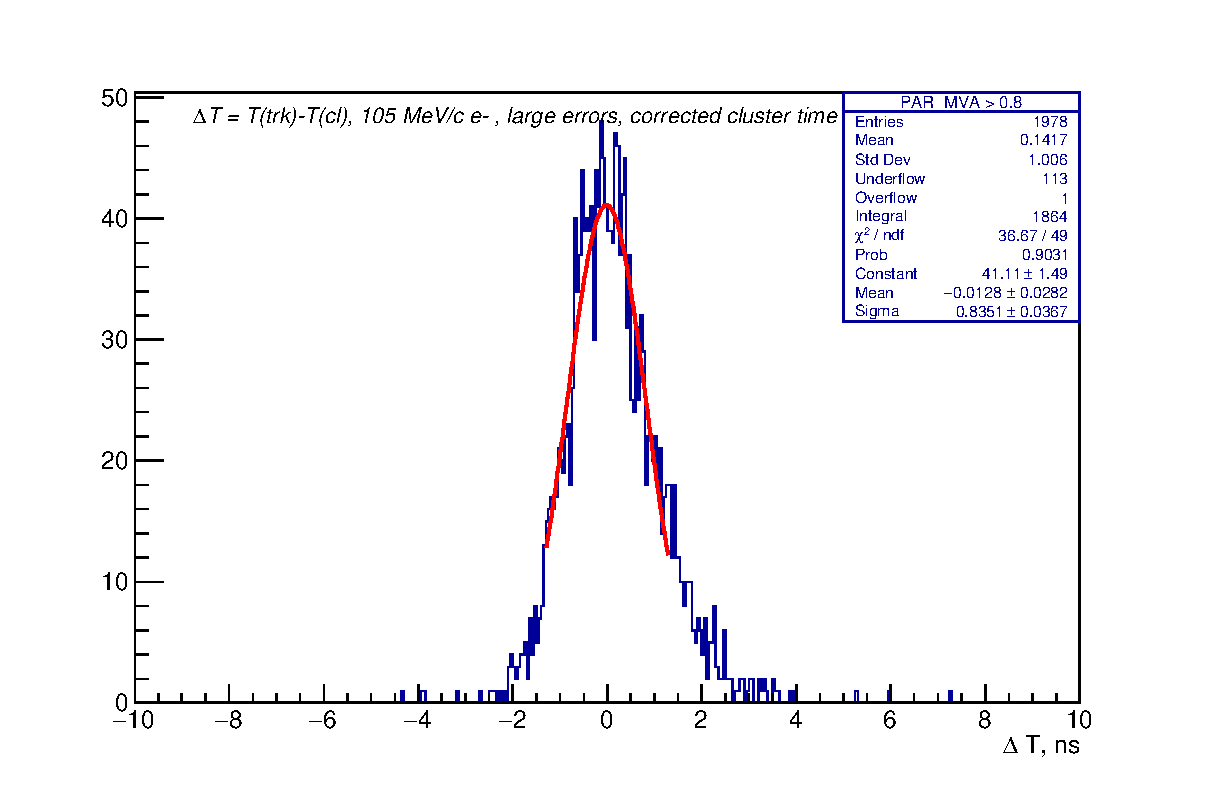
\includegraphics[width=0.64\textwidth]{figures/pdf/figure_00133_ele00s51b0_pid_emuana_trk_101_dt}
      % }
    };
    \node [text width=1cm, scale=0.8] at (3.,-2) {(c)};
    \node[anchor=south west,inner sep=0] at (10.7,-7.0) {
      % \node[shift={(0 cm,0.cm)},inner sep=0,rotate={90}] at (0,0) {}
      % \makebox[\textwidth][c] {
      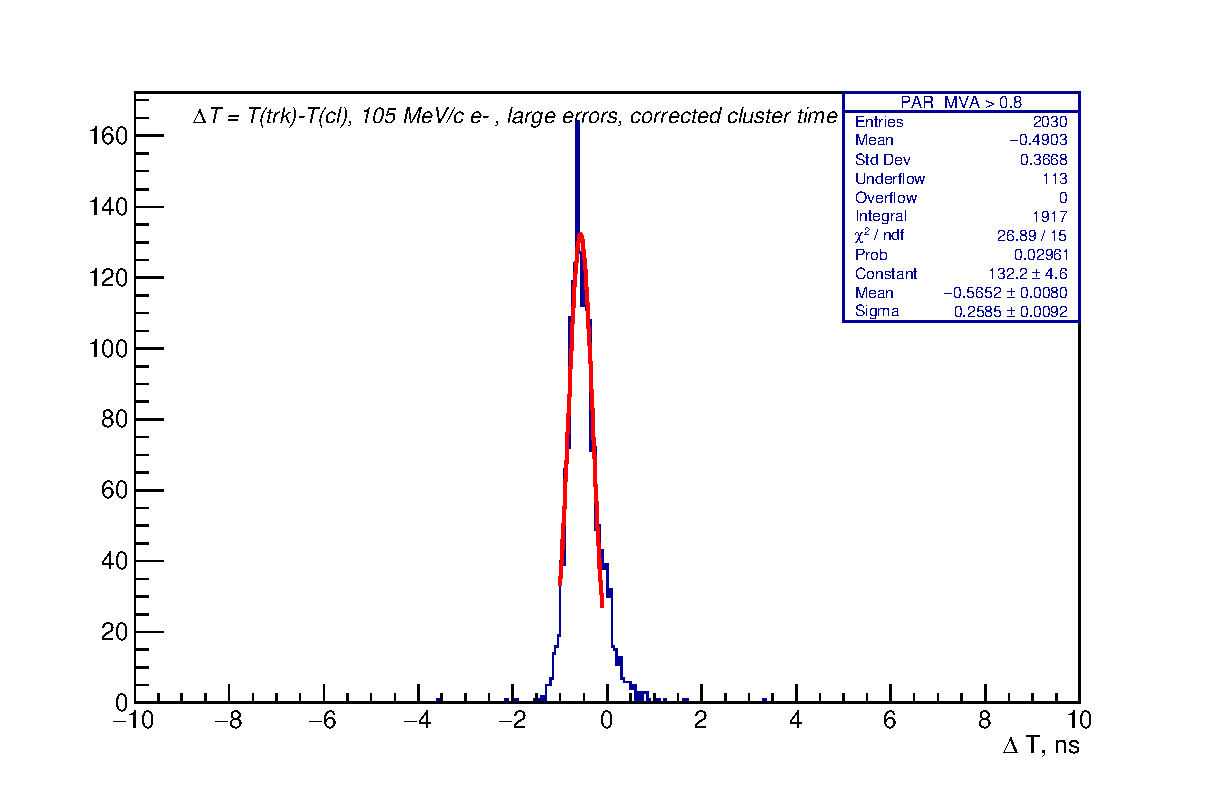
\includegraphics[width=0.64\textwidth]{figures/pdf/figure_00139_ele00s51b0_pid_emuana_trk_101_dt}
      % }
    };
    \node [text width=1cm, scale=0.8] at (13.7,-2) {(d)};
    % \node [text width=6cm, scale=0.8] at (4.5,6.4) {mu2e-18894 by Kevin Lynch and Jim Popp};
  \end{tikzpicture}
  % \captionof{figure} {
  \caption{
    \label{fig:track_cluster_dt}
    Track-cluster timing offsets and their correction: 
    (a) default offline configuration;
    (b) cluster assigned large errors in the fit; {\blue label (b) cluster large errors $\ra$ large errors}
    (c) cluster timing corrected by 1.6 ns, still large errors;
    (d) cluster timing corrected by 1.6ns, default errors {\blue label on plot (d) says large errors}
  }
\end{figure}



%%% Local Variables:
%%% TeX-master: "mu2e-36375"
%%% End:

%%% -*- mode:latex; mode:flyspell -*-

%%% Local Variables:
%%% TeX-master: "mu2e-36575"
%%% End:
\section{Tuning the calorimeter timing resolution}

The calorimeter timing simulation has been significantly improved since the Offline version
v9\_0\_5 used to start SU2020 branch.
The old timing simulation was largely underestimating the calorimeter timing resolution.
A better parametrization of the photon propagation time inside the crystal and, most significantly, a better implementation of the noise in the simulation in more recent versions of the Offline produces  simulation results much closer to the test beam measurements \cite{MU2E_35540_CALO_TIMING}.

The different components of the calorimeter noise during the first period of data taking have been estimated in \cite{MU2E_35519_CALO_NOISE} 
assuming the Run Plan reported in \cite{MU2E_33731_RUN1_PLAN}, where the results are summarized
in Table \ref{table:calonoise}. 
The noise components include the electronic noise (measured at the cosmic ray stand), 
radiation induced noise (RIN), and dark current due to neutron radiation damage
in the SiPMs (assuming an operation temperature of $-10^o$ C).
A safety factor of 2 has been used for the  neutron induced noise to reflect the uncertainty of the results of neutron radiation damage measurements.

\begin{table}[htbp]
  \begin{center} 
    \begin{tabular}{|c|c|c|c|c|}
      \hline
      Run 1 period      & FEE noise  & RIN     & Dark current noise & RIN$\oplus$Dark    \\ 
      \hline
      1 batch start     & 200 keV    & 280 keV &  --                & 344 keV  \\
      1 batch end       & 200 keV    & 280 keV &  450 keV           & 566 keV  \\
      2 batch end       & 200 keV    & 400 keV &  492 keV           & 634 keV  \\
      \hline
    \end{tabular}
  \end{center}
  \caption{
  \label{table:calonoise}
    Calorimeter noise levels in different Run 1 periods as estimated in \cite{MU2E_35519_CALO_NOISE}. 
  }
  % \vspace{0.5in}
\end{table}

Using the results in the Table \ref{table:calonoise}, we assume an average noise of 455 keV
for the 1 batch period and 600 keV for the 2 batch period. 
A parametrization of the time resolution as function of the RIN$\oplus$Dark noise level (assuming FEE noise fixed at 200 keV) and the energy deposited
in a crystal obtained using the latest calorimeter simulation software has been presented in  \cite{MU2E_36225_CALO_TIME_RES}.
The curves corresponding to a RIN$\oplus$Dark noise of 455 keV and 600 keV are the lower dashed
lines in Figures \ref{fig:calorimeter_timing_resolution_1batch} and  \ref{fig:calorimeter_timing_resolution_2batch}.

Table \ref{table:calonoise} does not include the time jitter of the accelerator signal.
This effect should also be included in the tracker timing simulation, where it is currently
ignored. For particle identification, the only relevant quantity is the relative time
between the tracker and calorimeter. 
We decided not to change the tracker timing simulation, but instead to add the accelerator
clock jitter only to the cluster time.
Preliminary measurements \cite{MU2E_35392_TIME_JITTER} show a time jitter of 172 ps
for a chain of 2 DTCs and 217 ps for a chain of 7 DTCs. We take 200 ps as our best estimate.

Integration of the latest updates to the calorimeter simulation software into the SU2020 branch
would be a task, very complicated technically. Instead, an additional Gaussian time smearing
component is added to the  CaloCrystalHitFromHit module to reproduce the desired time resolution. 

Figures \ref{fig:calorimeter_timing_resolution_1batch} and  \ref{fig:calorimeter_timing_resolution_2batch} show the output of the time resolution
simulation with the additional Gaussian smearing component as a function of the energy deposited
in the crystal for the two calorimeter disks for 1 and 2 batch modes.
The agreement with the expected analytical function is shown. 
The deviations at small energies are not important as the time resolution simulation
in those regions is known to be less reliable.

\begin{figure}[h]
%  \hspace{-0.6in}
  \begin{tikzpicture}
    \node[anchor=south west,inner sep=0] at (0.,0.) {
      % \node[shift={(0 cm,0.cm)},inner sep=0,rotate={90}] at (0,0) {}
      \makebox[\textwidth][c] {
        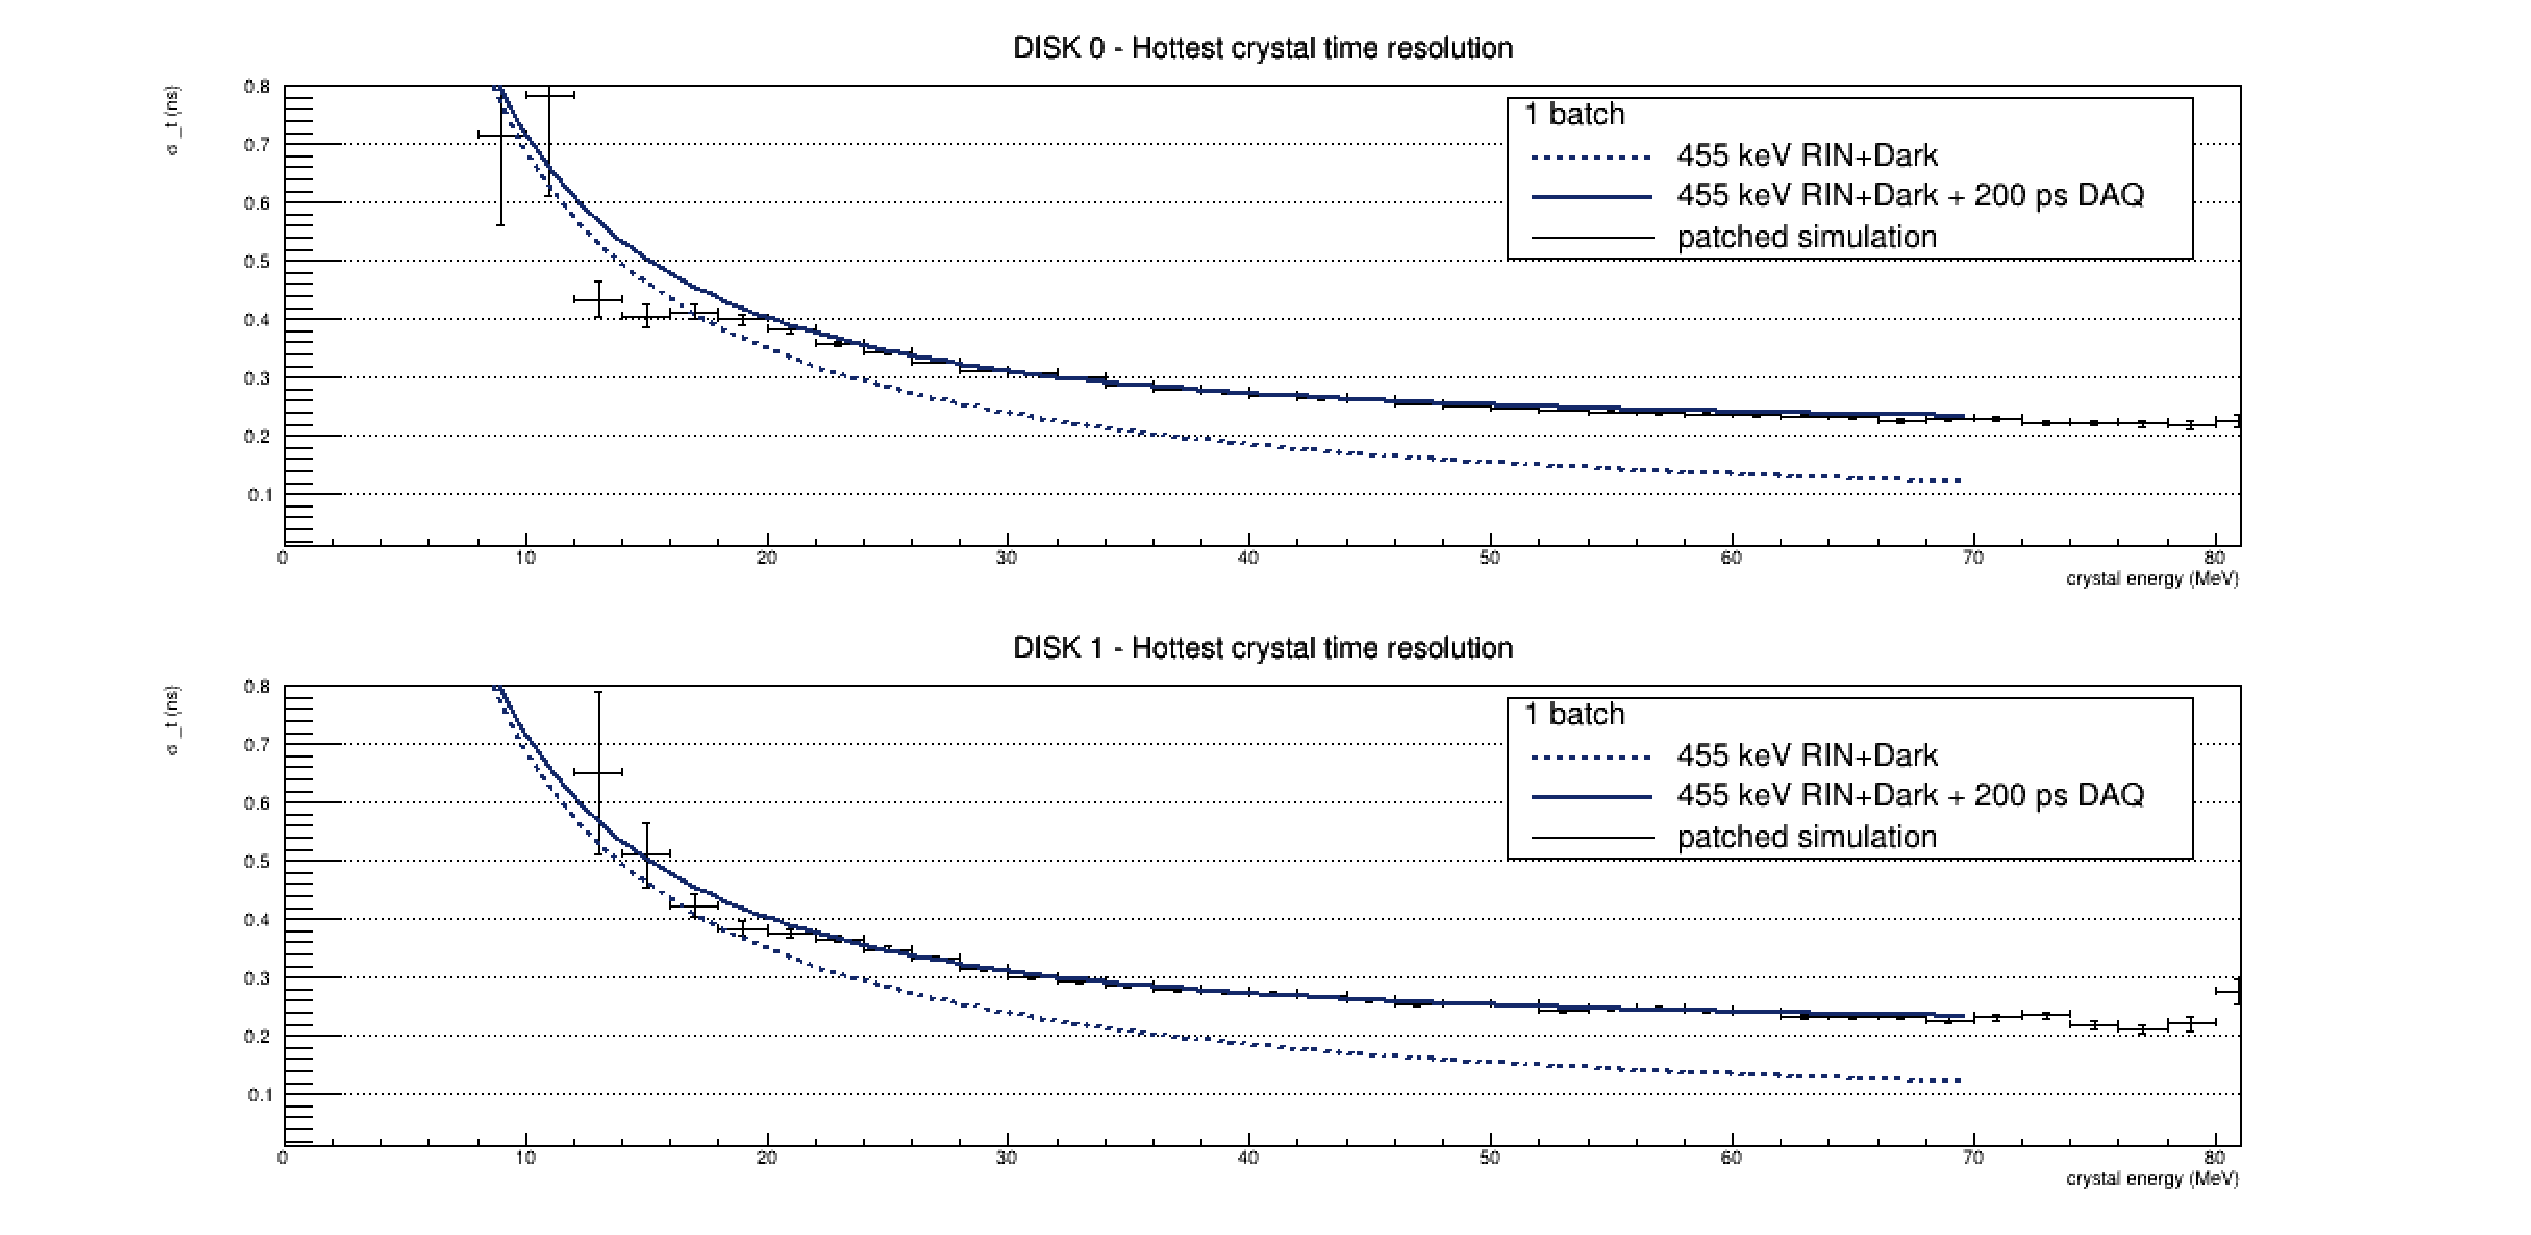
\includegraphics[width=0.90\textwidth, trim = 40 0 125 0, clip]{figures/pdf/figure_00401_sigmat_1batch_corrected}
      }
    };
    % \node [text width=6cm, scale=0.8] at (4.5,6.4) {mu2e-18894 by Kevin Lynch and Jim Popp};
  \end{tikzpicture}
  % \captionof{figure} {
  \caption{
    \label{fig:calorimeter_timing_resolution_1batch}
    Tuning of the calorimeter timing resolution for the 1 batch run period.
    The lower dashed curve corresponds to the parametrization given in 
    \cite{MU2E_36225_CALO_TIME_RES} using a noise of 455 keV.
    The upper dashed curve includes the 200 ps for the DTCs time jitter.
    The black points represent the results of the SU2020 patched calorimeter time simulation.
  }
\end{figure}

\begin{figure}[h]
%  \hspace{-0.6in}
  \begin{tikzpicture}
    \node[anchor=south west,inner sep=0] at (0.,0.) {
      % \node[shift={(0 cm,0.cm)},inner sep=0,rotate={90}] at (0,0) {}
      \makebox[\textwidth][c] {
        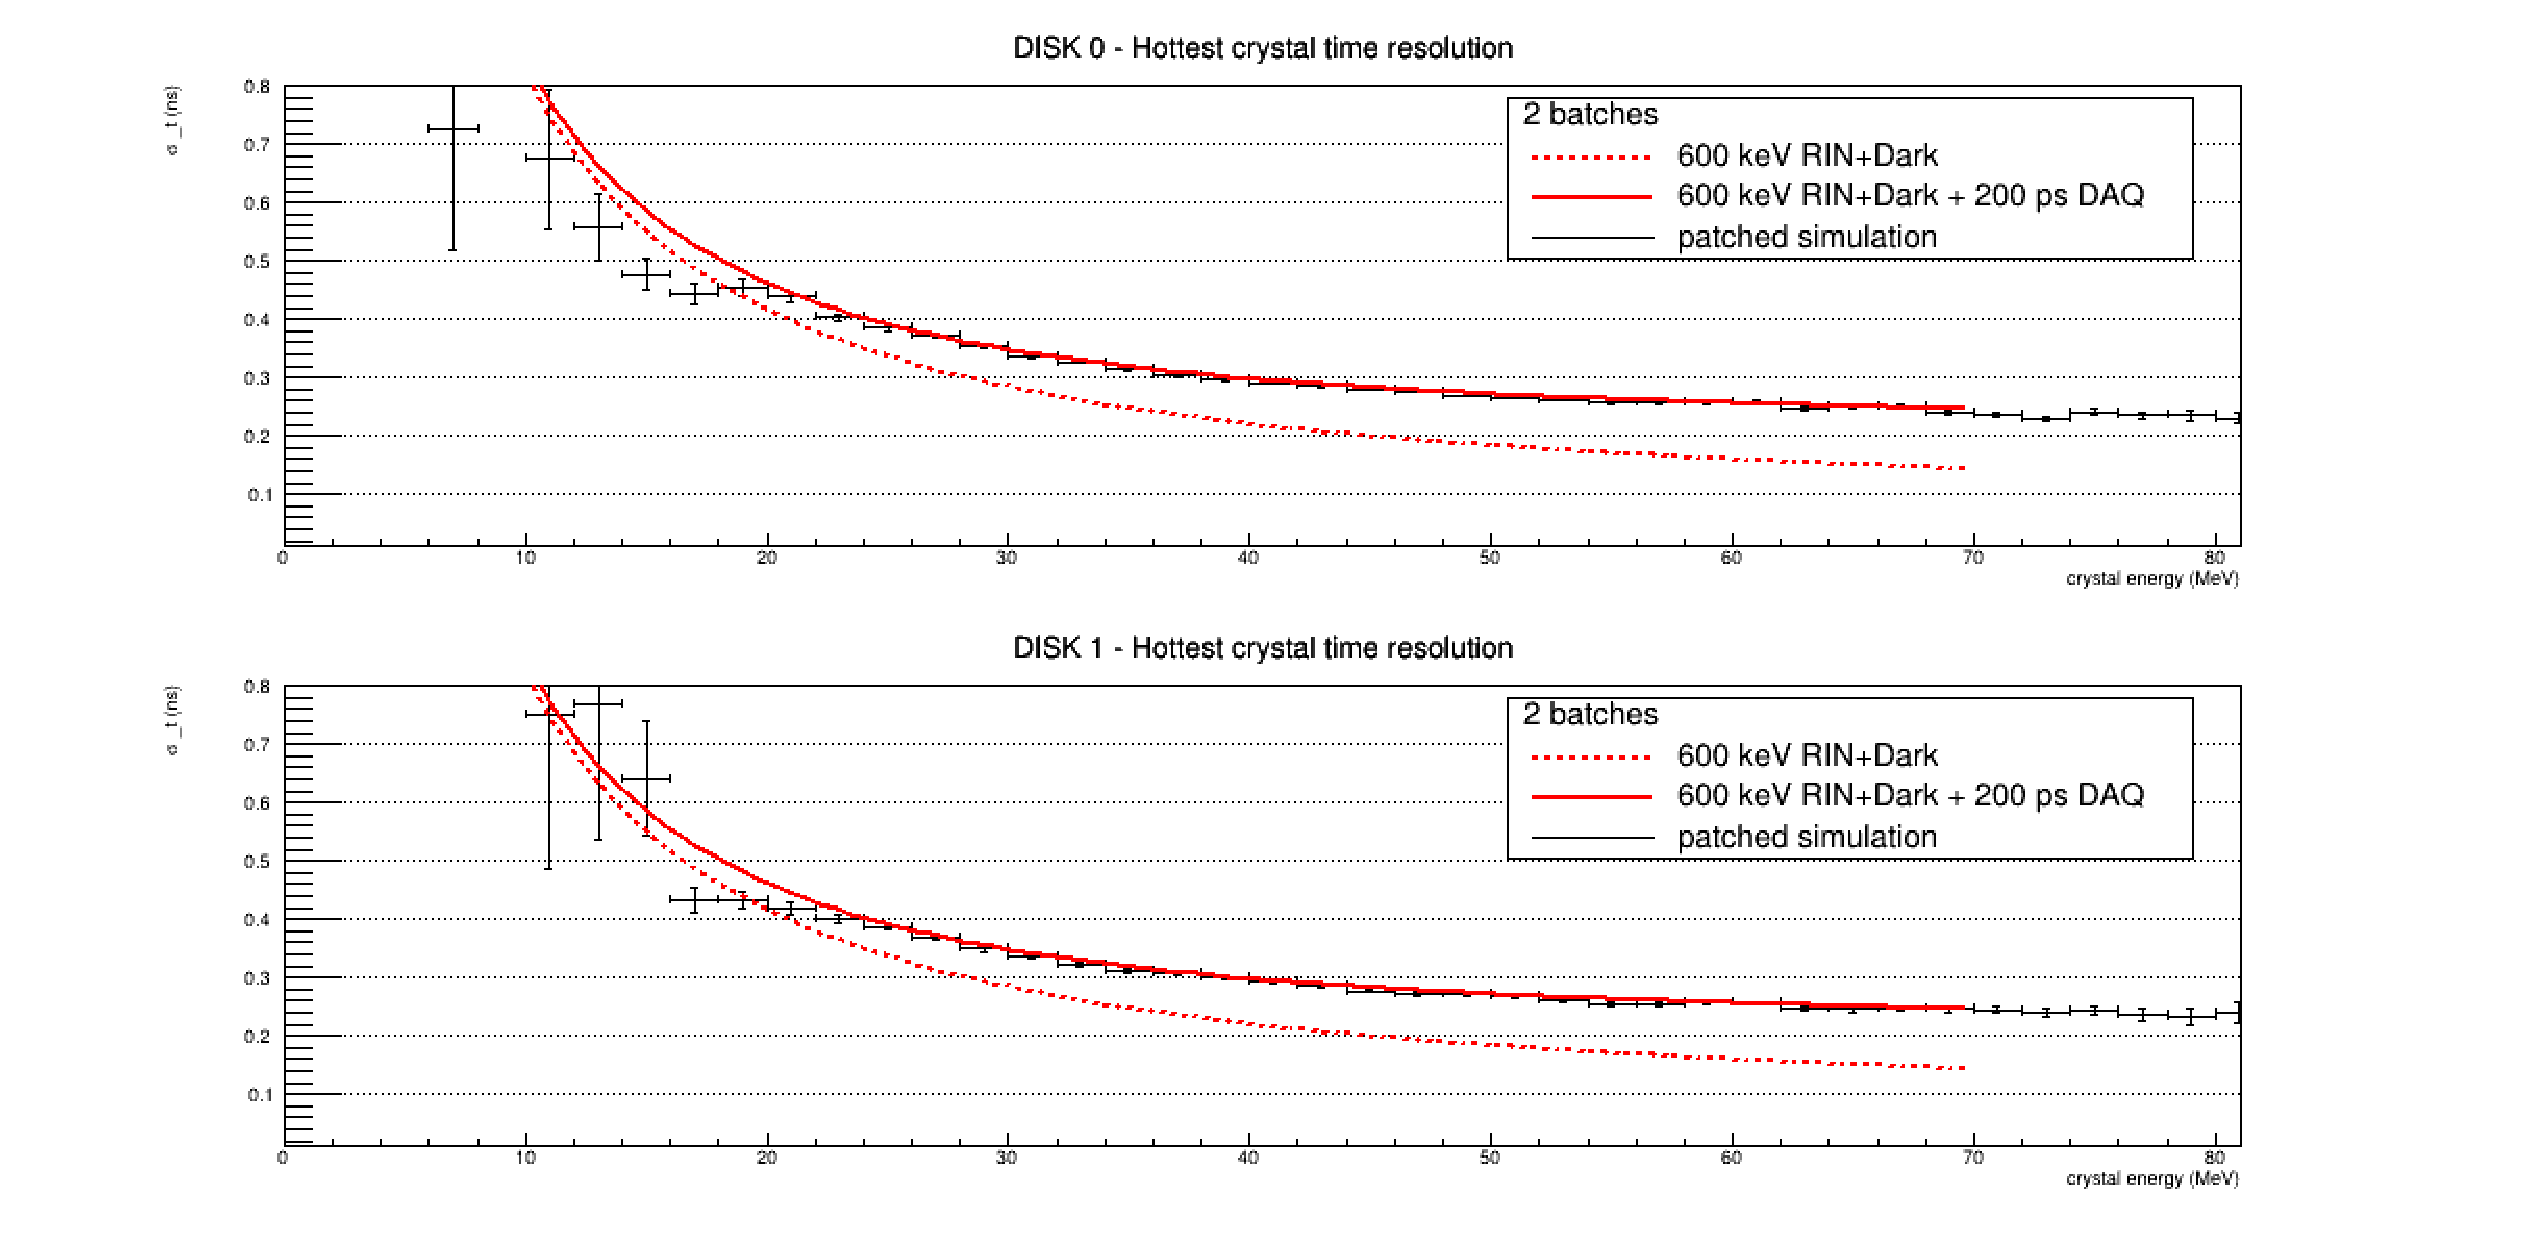
\includegraphics[width=0.90\textwidth, trim = 40 0 125 0, clip]{figures/pdf/figure_00402_sigmat_2batch_corrected}
      }
    };
    % \node [text width=6cm, scale=0.8] at (4.5,6.4) {mu2e-18894 by Kevin Lynch and Jim Popp};
  \end{tikzpicture}
  % \captionof{figure} {
  \caption{
    \label{fig:calorimeter_timing_resolution_2batch}
    Tuning of the calorimeter timing resolution for the 2 batch run period.
    The lower dashed curve corresponds to the parametrization
    given in \cite{MU2E_36225_CALO_TIME_RES} using a noise of 600 keV.
    The upper dashed curve includes the 200 ps for the DTCs time jitter.
    The black points represent the results of the SU2020 patched calorimeter time simulation. 
  }
\end{figure}

%%% mode: latex; mode:flyspell
%%%%%%%%%%%%%%%%%%%%%%%%%%%%%%%%%%%%%%%%%%%%%%%%%%%%%%%%%%%%%%%%%%%%%%%%%%%%% 
\section{Track momentum corrections}

The mean value of the reconstructed track momentum extrapolated to the tracker entrance is
slightly lower than the true MC momentum of the corresponding MC particle.
The offset is of the order of 30 keV/c and slightly different the track fits with different
ambiguity resolvers. 
We correct the reconstructed momenta of PAR tracks by 34 keV/c , and DAR tracks - by 30 keV/c.

\begin{figure}[h]
\hspace{-0.6in}
\begin{tikzpicture}
  \node[anchor=south west,inner sep=0] at (0,0.) {
    % \node[shift={(0 cm,0.cm)},inner sep=0,rotate={90}] at (0,0) {}
    % \makebox[\textwidth][c] {
      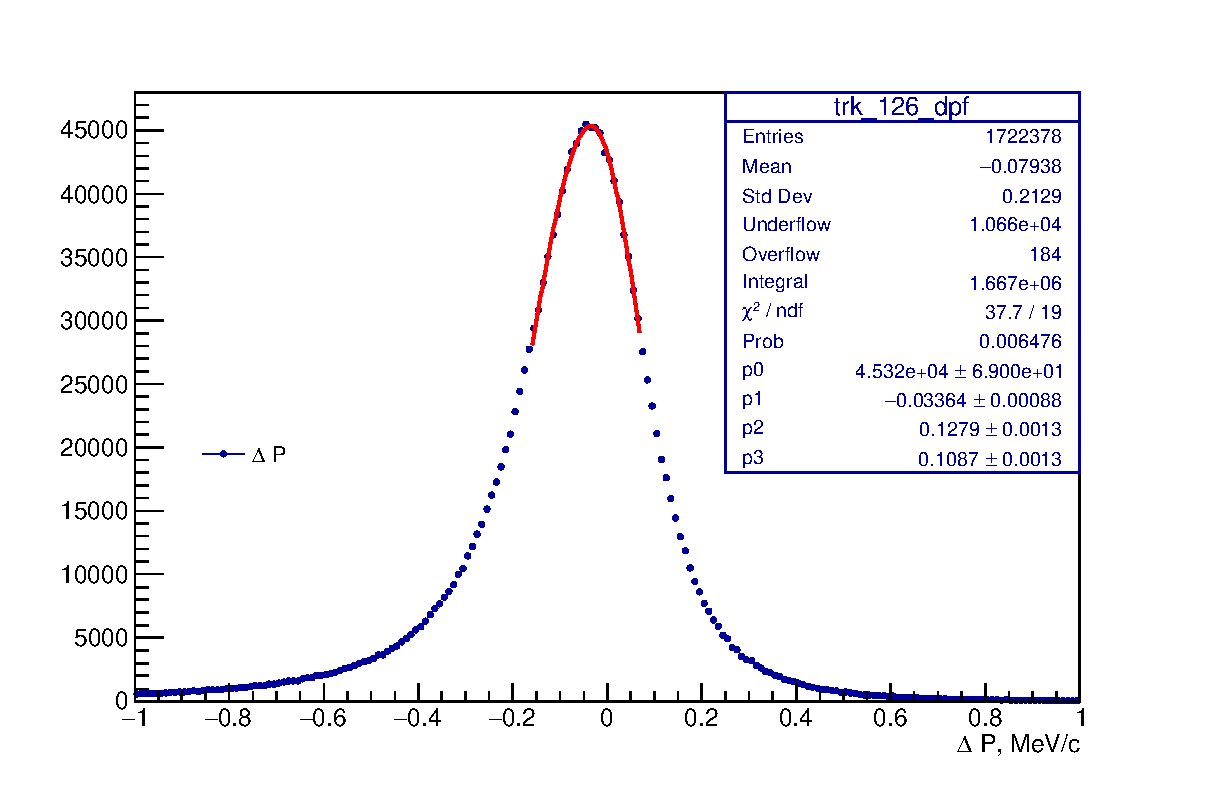
\includegraphics[width=0.65\textwidth]{figures/pdf/figure_00112_fele2s51b1_track_comp_ffff_1070_nocorr_trk_126_dpf}
    %}
  };
  \node[anchor=south west,inner sep=0] at (10,0.) {
    % \node[shift={(0 cm,0.cm)},inner sep=0,rotate={90}] at (0,0) {}
    % \makebox[\textwidth][c] {
      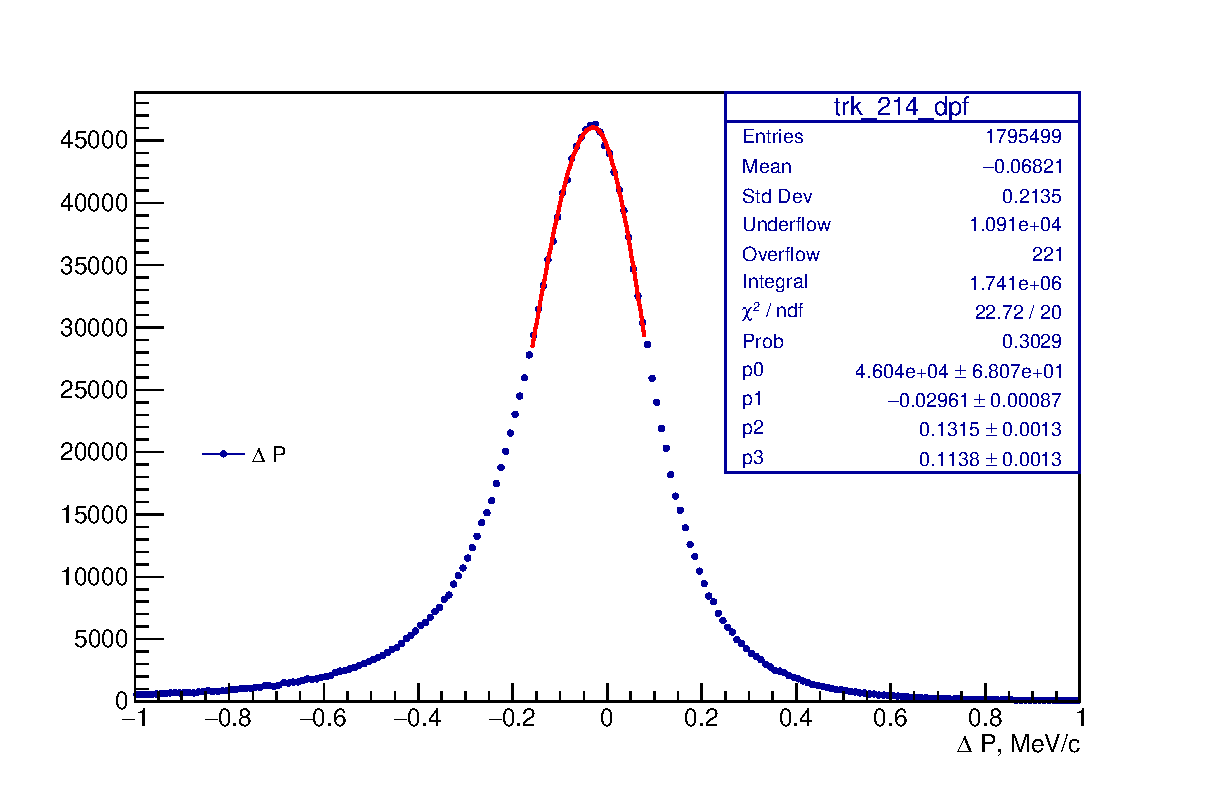
\includegraphics[width=0.65\textwidth]{figures/pdf/figure_00113_fele2s51b1_track_comp_ffff_1070_nocorr_trk_214_dpf}
    %}
  };
  % \node [text width=6cm, scale=0.8] at (4.5,6.4) {mu2e-18894 by Kevin Lynch and Jim Popp};
\end{tikzpicture}

\caption{
  \label{fig:sindrum_ii_fig_08_fit} 
  $\Delta P$ distributions at the tracker front for PAR (left) and DAR (right) tracks. The distributions  
  are fit with the asymmetric ($\sigma_{left} \ne \sigma_{right}$) gaussian function. Peak positions are used
  to correct the reconstructed  momenta of the tracks coming of the respective fits.
}
\end{figure}


%%% Local Variables:
%%% TeX-master: "mu2e-36575"
%%% End:

% -*- mode:flyspell; mode:latex  -*-

%%% Local Variables:
%%% TeX-master: "mu2e-36575"
%%% End:

%%%%%%%%%%%%%%%%%%%%%%%%%%%%%%%%%%%%%%%%%%%%%%%%%%%%%%%%%%%%%%%%%%%%%%%%%%%%% 
\section{Track quality selections}

%%%%%%%%%%%%%%%%%%%%%%%%%%%%%%%%%%%%%%%%%%%%%%%%%%%%%%%%%%%%%%%%%%%%%%%%%%%%%%
\subsection{\MuToEm\  channel}
\label{sec:mumem_channel}

Selection of correctly reconstructed tracks plays a critical role in the search, and 
to improve rejection of poorly reconstructed  tracks, an MVA-based technique is used.
A MLP ANN is trained to distinguish between correctly reconstructed tracks and mis-reconstructed
ones; good tracks are selected by requiring the ANN score to be above a certain value.

In the base version of the Mu2e Offline (v9\_0\_5) a track quality ANN has been trained only for PAR tracks,
we performed a similar training for the DAR tracks.
%
Following \cite{MU2E_4595_ANN_TRAINING}, we used the ROOT TMVA package to train an 
MLP ANN with 8 input variables and one hidden layer. The following eight variables
were used as inputs:

\begin{itemize}
\item
  {\bf na } : the number of active hits remaining on the track 
  after the Kalman fit and used in the calculation of the fit $\chi^2$
\item
  {\bf nafract} : the ratio of the number of active hits to the total number
  of hits (number of hits after the seed fit)
\item
  ${\bf log_{10}(fcons)}$ : {\bf fcons}, or the fit consistency, 
  is a probability-minded derivative of the track fit $\chi^2$. The logarithm
  of it is taken for numerical considerations
\item
  {\bf momerr} : the uncertainty on the reconstructed track momentum, returned by the fitter
\item
  {\bf t0err} : the uncertainty on the reconstructed track time, $T_0$, returned by the fitter
\item
  {\bf fda} : the fraction of doublet active hits over total number of active hits
\item
  {\bf fza } : the fraction of active hits with undefined drift direction
\item
  {\bf fma } : the fraction of straws with hits over the number of straws geometrically crossed by the track
\end{itemize}

The ANN training is aimed to optimize the separation of electron tracks reconstructed correctly, 
defined as $ |\Delta{P}| = |P_{reco}-P_{true}| < 0.25$ MeV/c, or approximately within $2\sigma$ of
the true value, from tracks with significantly larger reconstructed momentum, defined as
$\Delta{P} > 0.7$ MeV/c, or approximately $5\sigma$ above the true value.
%
Comparison between $P_{true}$ and $P_{reco}$ was performed in a plane corresponding to the tracker front.
%
Tracks with |D0| < 100 mm and 0.5 < \tandip < 1 were used to train the ANN.

To choose between the PAR-based and DAR-based fitters, we compared performance of the
trained DAR ANN to the performance of the default for the Mu2e Offline v9\_0\_5 PAR ANN.
%
We compared the performance of the two methods using the CD3 choice for the signal region:
103.85 < P < 104.90 MeV/c and $T_0 > 700$ ns.
%
Figure \ref{fig:mumem_ann_operational_point_choice} shows the expected DIO background plotted
versus the CE reconstruction efficiency. Both are plotted in relative units, normalized
to the DIO background and CE efficiency of the PAR track selection with the default
cut on the ANN score $S_{PAR} > 0.8$.
%
Square markers represent the PAR track selection and circle markers represent the DAR track selection;
red and black colors correspond to the conversion electron signal MC with 1 and 2 batch mode pileup 
datasets respectively.
%
In all cases the background model comes from the DIO-weighted fele2s51b1 dataset - 
flat energy electron MC with 1 batch mode pileup. 

As follows from Figure \ref{fig:mumem_ann_operational_point_choice},
using the DAR tracks increases the signal acceptance by 4-5\% with respect to PAR tracks for the same expected
background level. One can also see, that the Mu2e Offline default choice of the PAR ANN operational point
is quite close to the optimum - after the (1,1) point the PAR background starts increasing much faster than
the PAR signal, and the increase by 5\% comes along with a x2 higher DIO background.

For the DAR tracks, improving the signal acceptance by the same 5\% with respect to the default
Offline selection does not cost extra background. This determines the choices for the SU2020 analyses: 

\begin{itemize}
\item
  SU2020 analyses use DAR tracks
\item
  the ANN operational point corresponds to the cut on the output of $S_{DAR} > 0.2$.
\end{itemize}

\begin{figure}[H]
\begin{tikzpicture}
  \node[anchor=south west,inner sep=0] at (0,0.) {
    % \node[shift={(0 cm,0.cm)},inner sep=0,rotate={90}] at (0,0) {}
    \makebox[\textwidth][c] {
      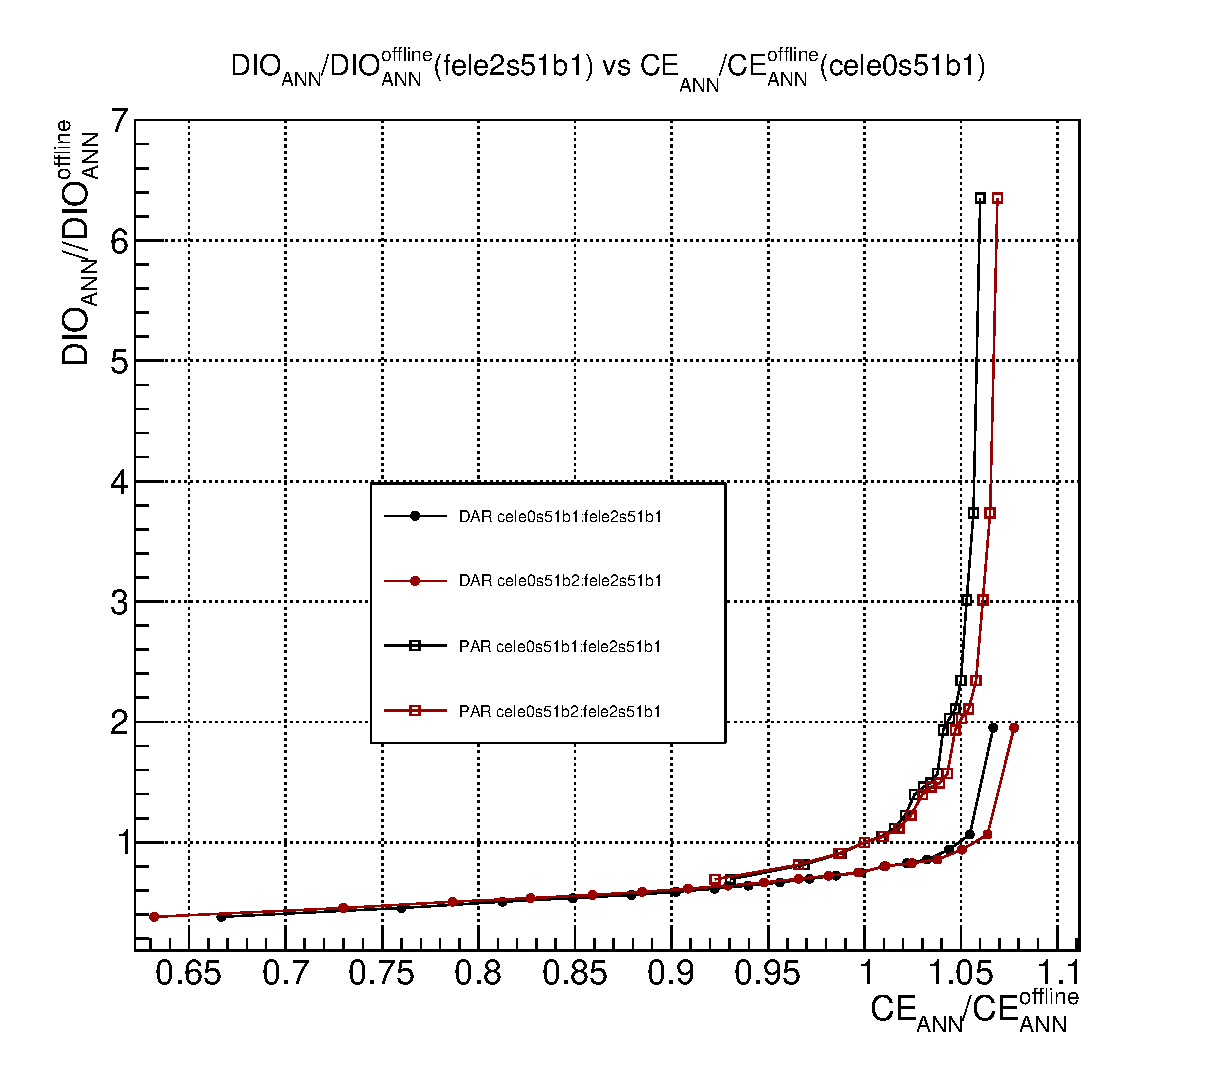
\includegraphics[width=0.8\textwidth]{figures/pdf/mumem_trq_ann_signal_vs_background}
    }
  };
  % \node [text width=6cm, scale=0.8] at (4.5,6.4) {mu2e-18894 by Kevin Lynch and Jim Popp};
\end{tikzpicture}
% \captionof{figure} {
\caption{
  \label{fig:mumem_ann_operational_point_choice}
%  \strike{Choice of the ANN operational point.}
  Relative DIO background versus relative signal acceptance.
  The expected DIO background, relative to the DIO background corresponding to the default Offline
  PAR ANN track selection,
  is plotted versus efficiency of the conversion electron signal acceptance, normalized to the efficiency
  of the signal selection using the default Offline PAR ANN.
  PAR curves, by construction, go through the point (1,1) which corresponds to default Offline PAR track selection
  of $S_{PAR} > 0.8$.
  Background : DIO-weighted {\bf fele2s51b1}, signal: {\bf cele0s51b1} (red), or {\bf cele0s61b2} (black).
}
\end{figure}

Figure \ref{fig:mumem_dar_vs_par_ann} compares the track momentum resolution distributions 
for DAR and PAR tracks reconstructed in the conversion electron plus two batch mode pile-up dataset,
{\bf cele0s61b2}, using either a fixed background or a fixed signal efficiency operational point. 
In Figure \ref{fig:mumem_dar_vs_par_ann}(a), the operational points for the DAR
and PAR track selections are chosen to give the same expected background -
in Figure \ref{fig:mumem_dar_vs_par_ann}(b), the same track selection efficiency. A higher 
high-momentum tail in the distribution for PAR tracks is clearly visible in both operational points.

\begin{figure}
\hspace{-0.6in}
\begin{tikzpicture}
  \node[anchor=south west,inner sep=0] at (0,0.) {
    % \node[shift={(0 cm,0.cm)},inner sep=0,rotate={90}] at (0,0) {}
    % \makebox[\textwidth][c] {
    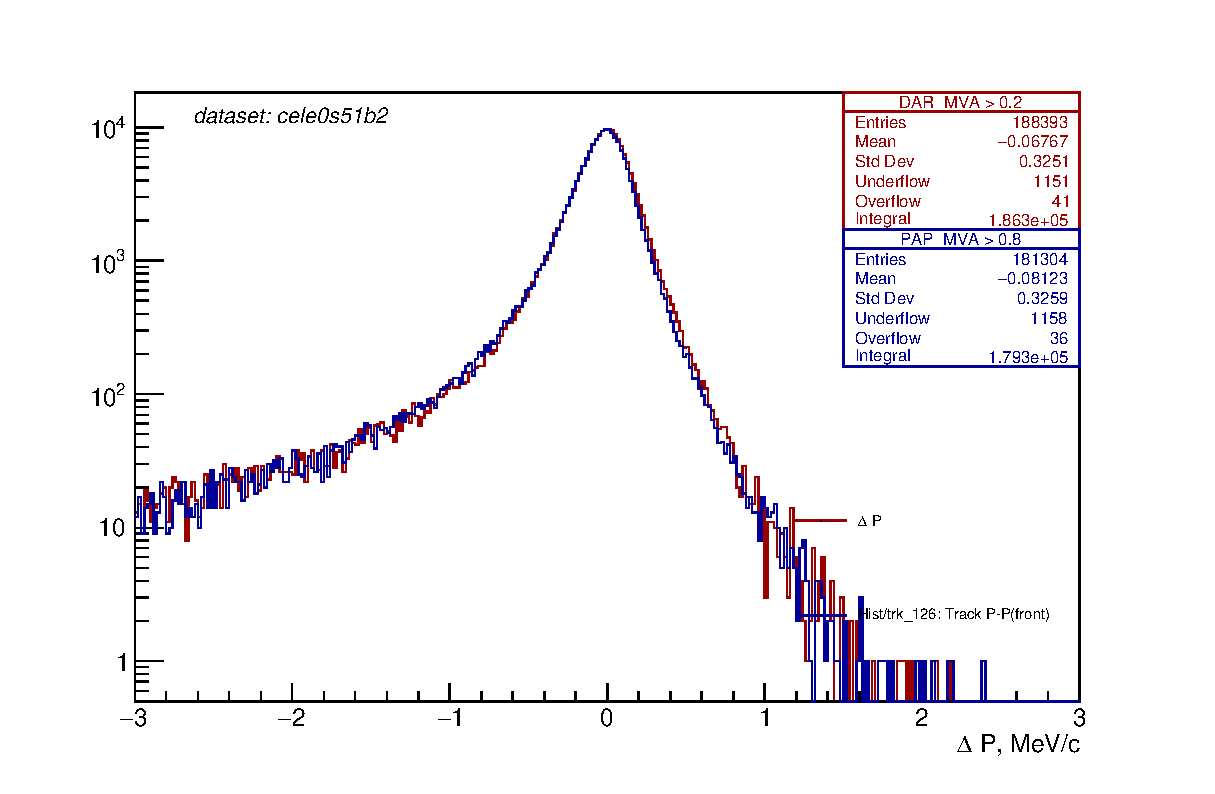
\includegraphics[width=0.64\textwidth]{figures/pdf/figure_00114_cele0s51b2_track_comp_ffff_1070_trk_214_vs_126_dpf}
    % }
  };
  \node [text width=1cm, scale=0.8] at (3.,4.5) {(a)};
  \node[anchor=south west,inner sep=0] at (10.5,0.) {
    % \node[shift={(0 cm,0.cm)},inner sep=0,rotate={90}] at (0,0) {}
    % \makebox[\textwidth][c] {
    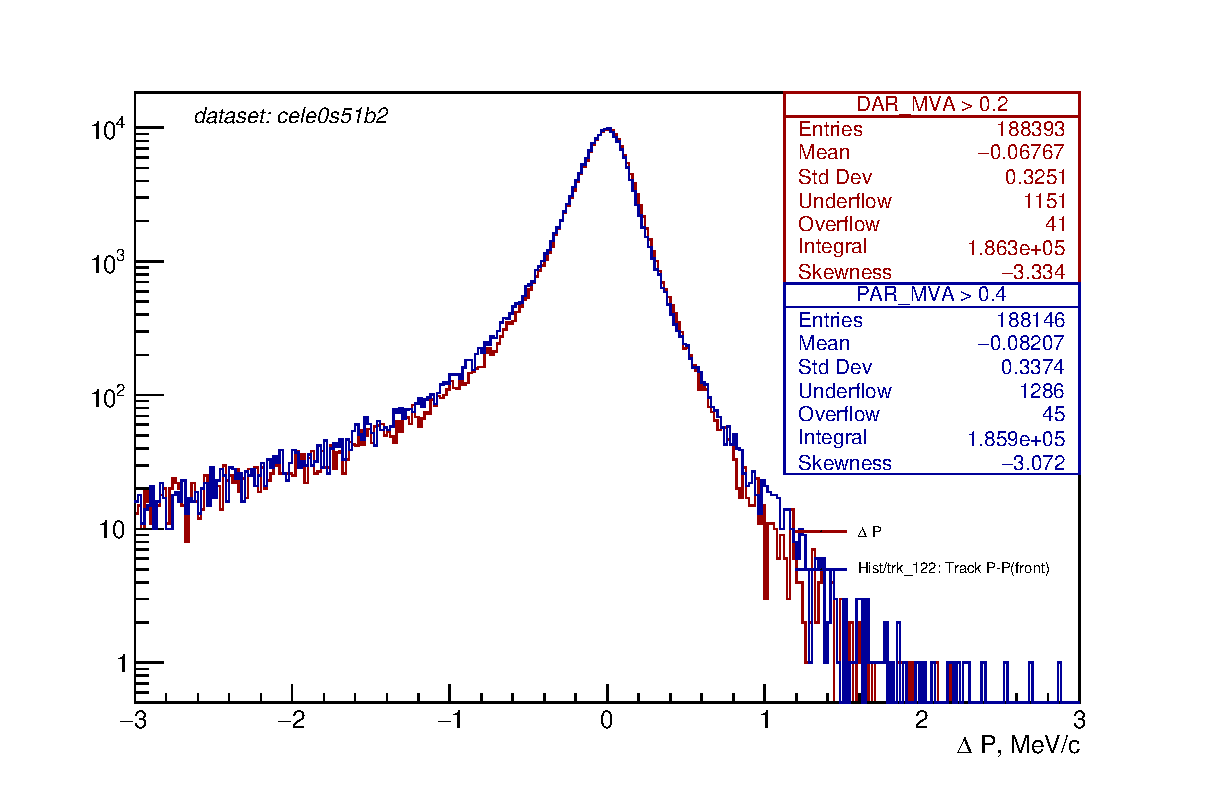
\includegraphics[width=0.64\textwidth]{figures/pdf/figure_00116_cele0s51b2_track_comp_ffff_1070_trk_214_vs_122_dpf}
    % }
  };
  \node [text width=1cm, scale=0.8] at (13.5,4.5) {(b)};
\end{tikzpicture}
% \captionof{figure} {
\caption{
  \label{fig:mumem_dar_vs_par_ann}
  DAR vs PAR track selection efficiency for two operational points: 
  (a): DAR ($S_{DAR} > 0.2$) and PAR ($S_{PAR} > 0.8$) selections correspond to the same background level ;  
  (b): DAR ($S_{DAR} > 0.2$) and PAR ($S_{PAR} > 0.4$) track selections correspond to the same efficiency
  The right-side tail, the most severely mis-reconstructed tracks, is a measure of the track selection
  quality.
}
\end{figure}

Improvements in the track reconstruction, for the same selection efficiency, result in significantly improved
rejection of mis-reconstructed tracks. Figure \ref{fig:dio_delta_p_1036_1050} shows the $\Delta{P}$ distribution
for the simulated DIO electrons (DIO-weighted {\bf fele2s51b1}) with reconstructed track momentum in [103.6, 105.0] MeV/c.
From that distribution one can easily see the importance of the relative contribution
of tracks with $\Delta{P}$ above a certain threshold. In particular, tracks with significantly mis-reconstructed
momentum, $\Delta{P} > 0.5$ MeV, represent about 0.23 of the expected DIO background (which is about 50\% lower
than the previous estimate of 0.355 for the same momentum window in \cite{MU2E_4595_ANN_TRAINING}).

\begin{figure}
  \begin{tikzpicture}
    \node[anchor=south west,inner sep=0] at (0,0.) {
      % \node[shift={(0 cm,0.cm)},inner sep=0,rotate={90}] at (0,0) {}
      \makebox[\textwidth][c] {
        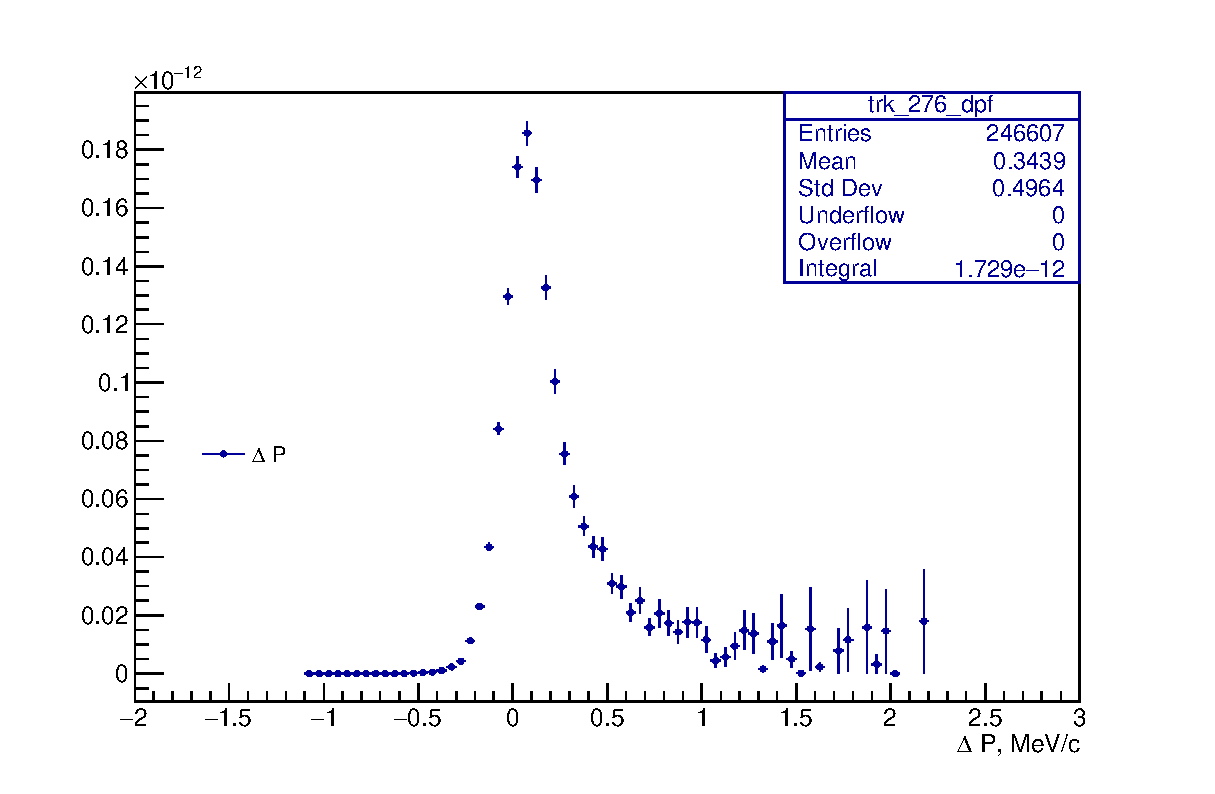
\includegraphics[width=0.99\textwidth]{figures/pdf/figure_00111_fele2s51b1_track_comp_ffff_1070_trk_276_dpf}
      }
    };
    % \node [text width=6cm, scale=0.8] at (4.5,6.4) {mu2e-18894 by Kevin Lynch and Jim Popp};
  \end{tikzpicture}
  % \captionof{figure} {
  \caption{
    \label{fig:dio_delta_p_1036_1050} 
    $\Delta P ~=~ P_{reco} -P_{true}$ distribution for the simulated DIO background in the region [103.6,105.0] MeV.
    77.2\% of the reconstructed events in this region are expected to have $\Delta P < 0.5$ MeV/c
  }
\end{figure}

As a cross-check, we used the TMVA package to train a BDT-based track quality classifier.
Similar to \cite{MU2E_33150_ANN_TRAINING}, we found that the MLP ANN performed slightly better,
so the current analysis uses a MLP ANN-based track quality selection. 
To explore the parameter space, the definition of a ``mis-reconstructed track'' has been varied
and a similar ANN has been trained to discriminate tracks reconstructed with $|\Delta{P}| < 0.25$ MeV/c 
from tracks with $\Delta{P} > 0.6$ MeV/c.
No improvement in the DIO suppression in the region [103.85, 104.9] MeV/c was observed. 

%%%%%%%%%%%%%%%%%%%%%%%%%%%%%%%%%%%%%%%%%%%%%%%%%%%%%%%%%%%%%%%%%%%%%%%%%%%%%%
\newpage
\subsection{\MuToEp\ channel}
\label{sec:mumep_channel}

To select tracks in the \MuToEp\ channel, a conversion positron MC with one-batch mode pileup dataset
({\bf cpos0s51b1}) has been used to train an MLP ANN to discriminate between well reconstructed and
mis-reconstructed positron tracks.
%
The ANN configuration and the definitions of well reconstructed and mis-reconstructed tracks are
the same as described in Section \ref{sec:mumem_channel}.

Figure \ref{fig:mumep_trq_ann} compares the expected background vs the signal efficiency curves,
relative to the default Offline positron selection (as in Figure \ref{fig:mumem_ann_operational_point_choice}),
for PAR (squares) and DAR  (circles) tracks. The background definition, however, is different.
Unlike in \MuToEm\ channel, in \MuToEp\ channel there is no well defined background process whose contribution
could be used as a measure of mis-reconstruction. 
The RMC contribution depends on the assumptions about the RMC photon momentum distribution and,
in particular, its endpoint. Because of this, the background in Figure \ref{fig:mumep_trq_ann} 
is defined as the expected number of events with mis-reconstructed momentum $\Delta{P} > 1.0$ MeV.
%
The signal is integrated over the [90.5,92.5] MeV/c momentum window.

Figure \ref{fig:mumep_trq_ann}.(b) shows the same performance curves as Figure \ref{fig:mumep_trq_ann}.(a),
but with the vertical axis in logarithmic scale. It is interesting to see that for a given background
definition, the background increases exponentially with the signal acceptance for both types of tracks.
For the same signal acceptance, the ANN-based selection of DAR tracks results in lower
backgrounds, so the sensitivity estimate in the \MuToEp\ channel also uses the DAR tracks.

For the choice of the operational point, the cut $S_{DAR} > 0.2$ improves the signal acceptance
by 10\%, while increasing the background by 15\%. Relaxing the cut and moving the cut value to $S_{DAR} > 0.15$
adds another 2\% to the CP acceptance, while the background grows much faster and
becomes $B_{DAR}/B_{PAR}^{default} = 1.5,$ Thus, the default cut on $S_{DAR}^+$ is the same as
in the electron channel:  $S_{DAR}^+ > 0.2$

An attempt to train a similar ANN for PAR tracks didn't result in an improvement of an ANN-based track
selection. As the training parameters in both cases are essentially the same, this result is somewhat 
surprising and may be pointing to a potential of further improvements. 

\begin{figure}[H]
  \hspace{-0.6in}
  \begin{tikzpicture}
    \node[anchor=south west,inner sep=0] at (0,0.) {
      % \node[shift={(0 cm,0.cm)},inner sep=0,rotate={90}] at (0,0) {}
      % \makebox[\textwidth][c] {
      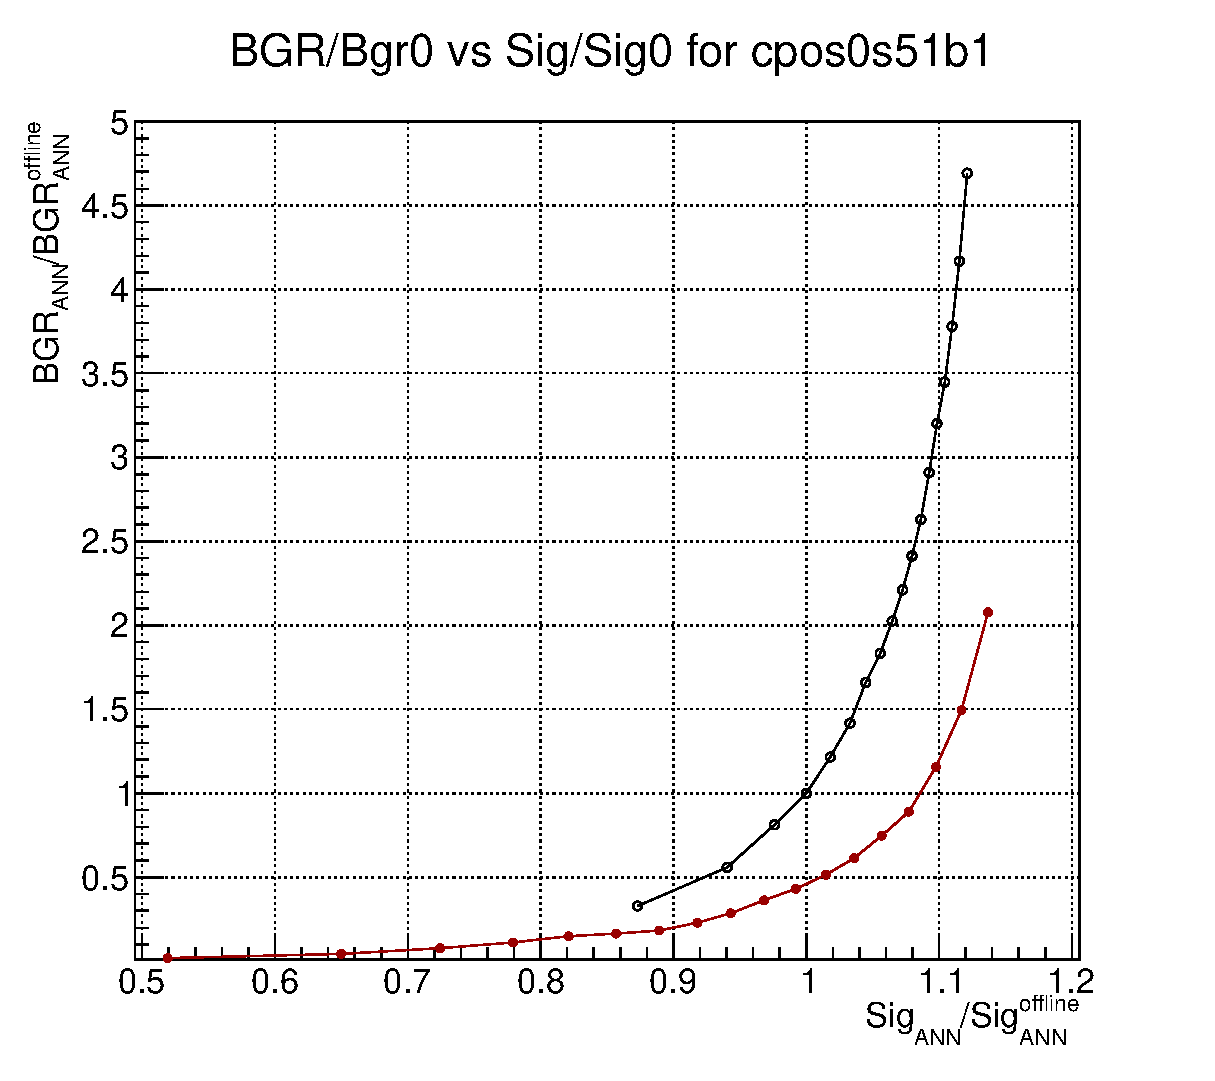
\includegraphics[width=0.55\textwidth]{figures/pdf/mumep_trq_ann_signal_vs_background_lin}
      % }
    };
    \node [text width=1cm, scale=1.0] at (3.,3.5) {(a)};
    \node[anchor=south west,inner sep=0] at (10,0.) {
      % \node[shift={(0 cm,0.cm)},inner sep=0,rotate={90}] at (0,0) {}
      % \makebox[\textwidth][c] {
      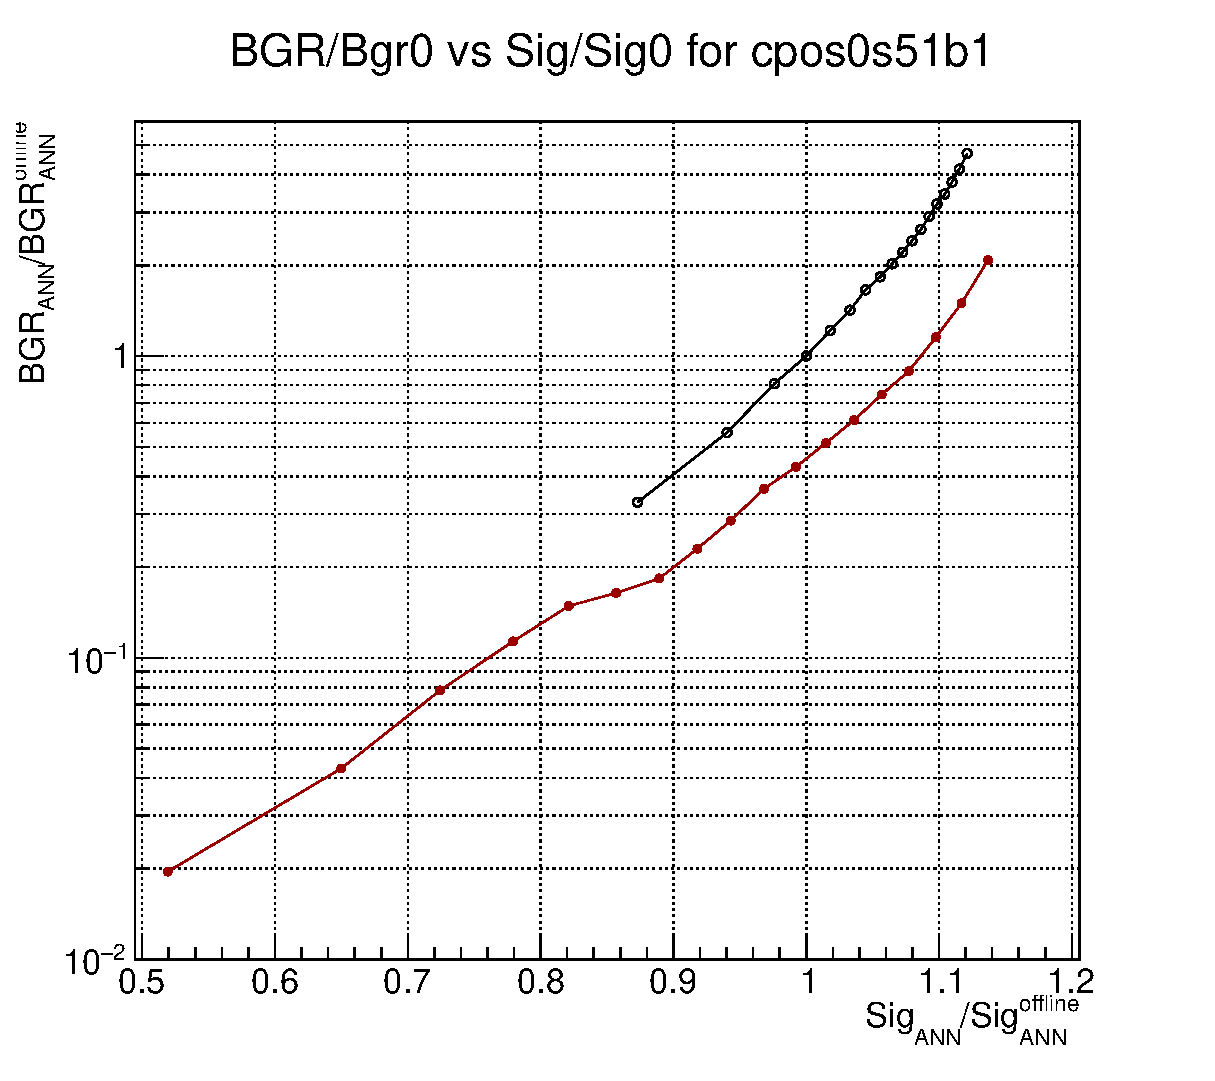
\includegraphics[width=0.55\textwidth]{figures/pdf/mumep_trq_ann_signal_vs_background_log}
      % }
    };
    \node [text width=1cm, scale=1.0] at (13.,3.5) {(b)};
  \end{tikzpicture}
  % \captionof{figure} {
  \caption{
    \label{fig:mumep_trq_ann} 
    DAR (Circles) vs PAR (squares) background vs signal window efficiency.
    Signal: {\bf cpos0s51b1}, 90.5 < P < 92.5 MeV/c ;
    background:{\bf cpos0s51b1} , tracks with $\Delta{P} > 1.0$ MeV.
    Both signal and background are measured in units of signal and background efficiency
    corresponding to the selection using the default Offline v9\_0\_5 ANN-based track
    selection, $S_{PAR}^+ > 0.8$.
  }
\end{figure}

%%%%%%%%%%%%%%%%%%%%%%%%%%%%%%%%%%%%%%%%%%%%%%%%%%%%%%%%%%%%%%%%%%%%%%%%%%%%%%
\subsection{Testing charge symmetry of the ANN-based track selection}

It is worth noting that the track parameters used for ANN training do not depend explicitly
on the reconstructed track sign. One could therefore expect the efficiency of the ANN-based
track selection to be charge-symmetric. To check this hypothesis, Figure \ref{fig:su2020_mva_test_dar}
compares the efficiency of the electron trained ANN-based selection for 105 MeV electrons and 105 MeV positrons.

Figure \ref{fig:su2020_mva_test_dar} confirms that for the same track momentum, the ANN-based selection
is charge-symmetric with an accuracy better than 0.5\%. The third, and the only visible, distribution
in Figure \ref{fig:su2020_mva_test_dar} corresponds to 105 MeV electron tracks selected
using the ANN trained on 92 MeV positrons as described in Section \ref{sec:mumep_channel}. One would expect
the efficiency of this selection to be sub-optimal, but rather surprisingly, the efficiency is reduced by
less than 4\%.
Observed charge symmetry allows to use one common ANN, trained using 105 MeV/c tracks, for track selection
in all \MuToEm\ search analyses and another common ANN, trained using 92 MeV/c tracks, for track selection 
in all \MuToEp\ search analyses.

\begin{figure}
  % \hspace{-0.6in}
  \begin{tikzpicture}
    \node[anchor=south west,inner sep=0] at (0,0.) {
      % \node[shift={(0 cm,0.cm)},inner sep=0,rotate={90}] at (0,0) {}
      \makebox[\textwidth][c] {
        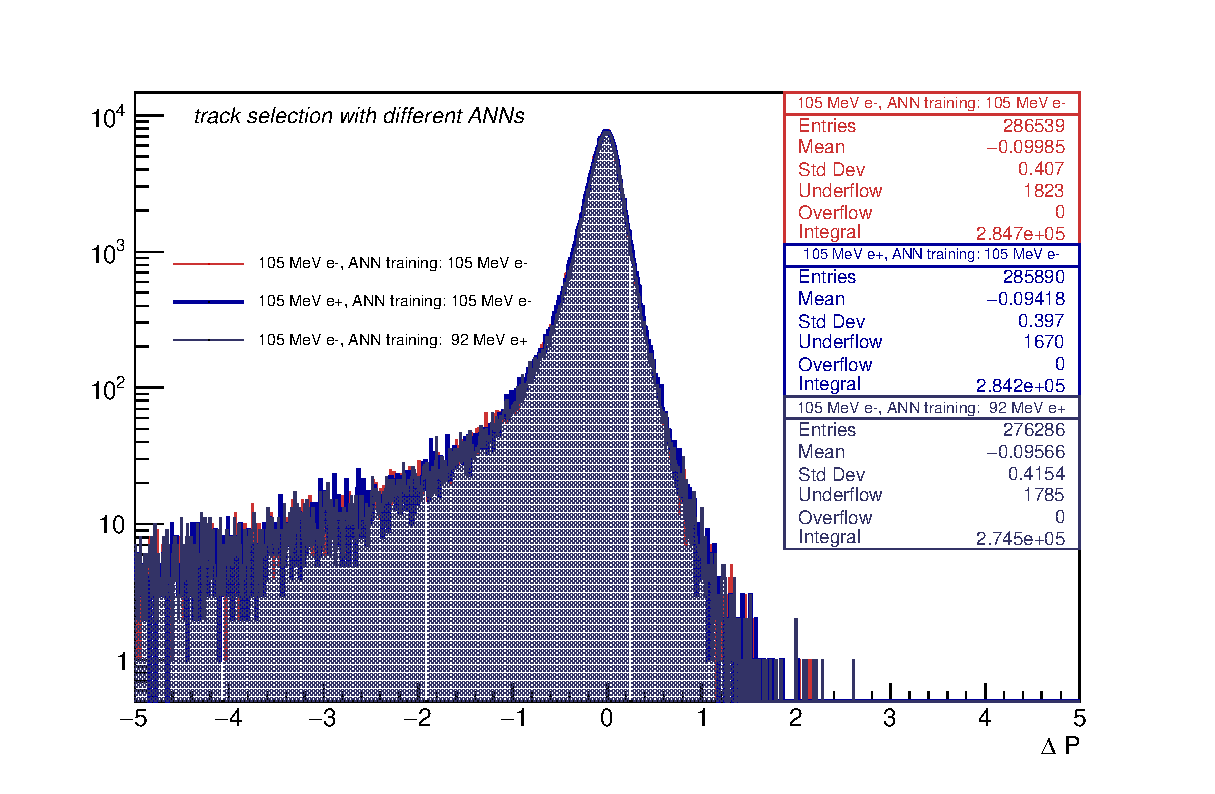
\includegraphics[width=0.95\textwidth]{figures/pdf/figure_00231_su2020_mva_test_dar}
      }
    };
    % \node [text width=6cm, scale=0.8] at (4.5,6.4) {mu2e-18894 by Kevin Lynch and Jim Popp};
  \end{tikzpicture}
  % \captionof{figure} {
  \caption{
    \label{fig:su2020_mva_test_dar} 
    105 MeV/c electrons and positrons selected using an ANN trained on 105 MeV/c electrons,
    and 105 MeV/c electrons selected using an ANN trained on 92 MeV/c positrons
  }
\end{figure}


%%%%%%%%%%%%%%%%%%%%%%%%%%%%%%%%%%%%%%%%%%%%%%%%%%%%%%%%%%%%%%%%%%%%%%%%%%%%%%
\subsection{Track selection cuts summary}
\label{sec:track-selection_cuts_summary}
  
For SU2020 analyses, a well reconstructed track is a DAR track satisfying the following requirements:

\begin{itemize}
\item
  the track impact parameter, ${\bf d_0}$, is consistent with the track coming from the stopping target: 
  ${\bf |d_0|} < 100$ mm. We note that ${\bf d_0}$ is calculated at a point of closest approach of
  the reconstructed trajectory to the beam axis, which is located inside the Mu2e tracker and 
  % {\blue which point inside the tracker?} - point of the trajectory closest approach to the beam axis
  several meters away from the stopping target,
  and therefore cannot be directly compared with the radius of the stopping target foils ;
\item 
  the track dip angle, $\lambda = 90^o - \alpha$, where $\alpha$ is the track angle with respect 
  to the solenoid axis, is within $ 0.5 < \tan{\lambda} < 1$. 
  The choice of the lower cutoff value, 0.5, is not currently dictated by any real considerations.
  It is a clean-up cutoff, which does not introduce any visible inefficiency. 
  The requirement $\tan{\lambda} < 1$ reduces the tracking acceptance by about 10\%, 
  and, most importantly, is an anti-cosmics selection. This cut also rejects tracks of particles 
  produced upstream of the stopping target, i.e. coming from the TS ; 
\item
  track quality ANN score $S_{ANN} > 0.2$ ;
\item
  number of the active track hits $N_{\rm active} >= 20$ ;
\item
  a calorimeter cluster is included into a track fit and is not rejected by the fitter. For ntuple-level analyses,
  this requirement is implemented by requiring the fit error $\sigma_{T0} < 0.9$ ns.
  The implementation is approximate: in the fit, the calorimeter cluster is assigned $\sigma_T ~=~ 0.5$ ns,
  so tracks with $\sigma_{T0} > 0.9$ ns are likely to have the calorimeter cluster rejected .
  The effect of the cut is shown in Figure \ref{fig:sigt0_1_and_rmax_1}(a);
\item
  $R_{max} ~<~ 680$ mm . The distributions $R_{max}$ for CE and electrons reconstructed in cosmics-induced events
  are shown in Figure \ref{fig:sigt0_1_and_rmax_1}(b);

\end{itemize}

\begin{figure}
  \hspace{-0.6in}
  \begin{tikzpicture}
    \node[anchor=south west,inner sep=0] at (0,0.) {
      % \node[shift={(0 cm,0.cm)},inner sep=0,rotate={90}] at (0,0) {}
      % \makebox[\textwidth][c] {
      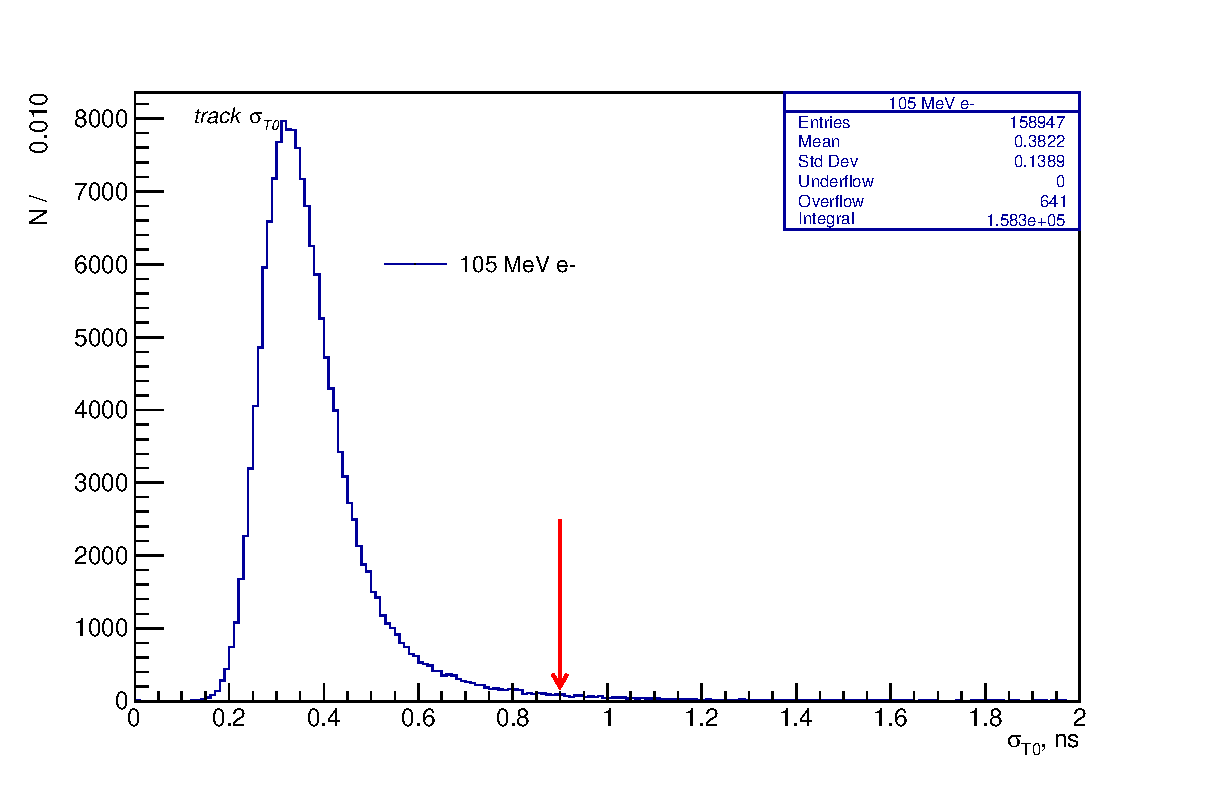
\includegraphics[width=0.60\textwidth]{figures/pdf/figure_00233_tid_1_t0err_1}
      % }
    };
    \node[anchor=south west,inner sep=0] at (11.,0.) {
      % \node[shift={(0 cm,0.cm)},inner sep=0,rotate={90}] at (0,0) {}
      % \makebox[\textwidth][c] {
      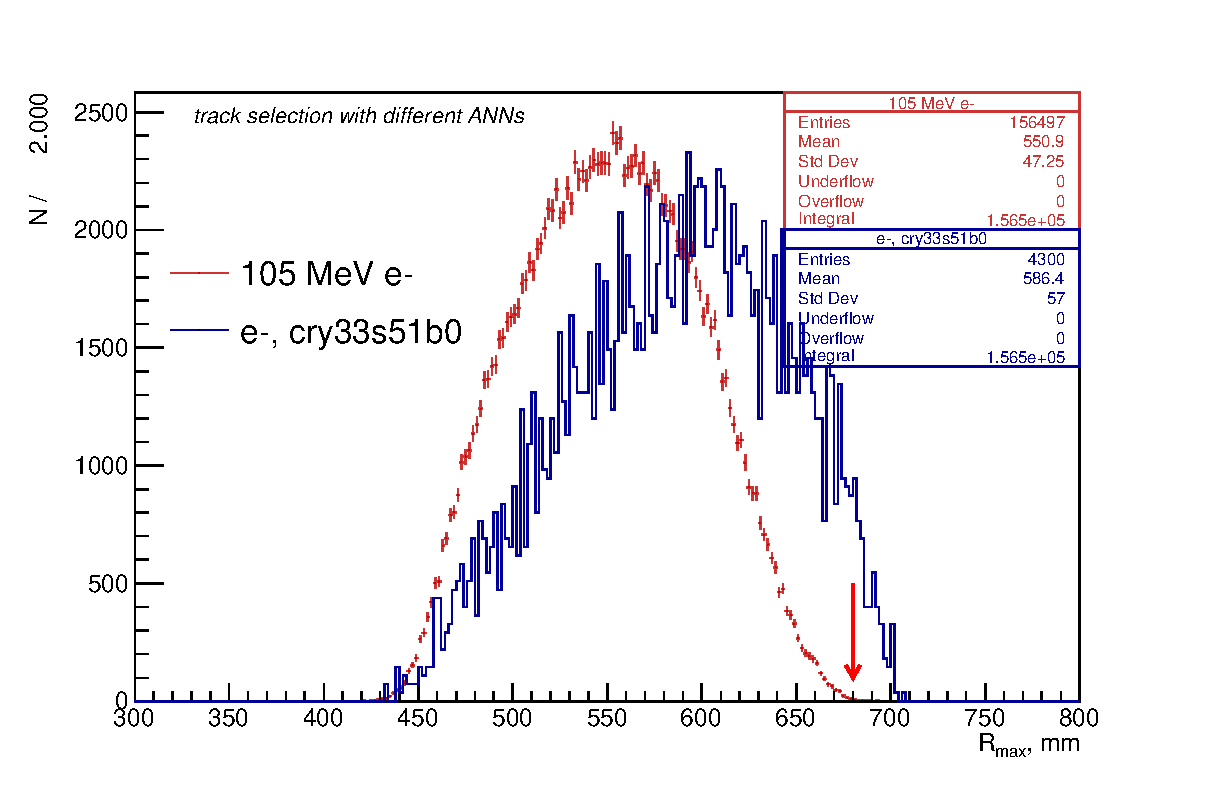
\includegraphics[width=0.60\textwidth]{figures/pdf/figure_00232_tid_1_rmax_1}
      % }
    };
    \node [text width=1cm, scale=0.8] at ( 2.5,5.4) {(a)};
    \node [text width=1cm, scale=0.8] at (13.5,5.4) {(b)};
  \end{tikzpicture}
  % \captionof{figure} {
  \caption{
    \label{fig:sigt0_1_and_rmax_1}
    (a): $\sigma_{T0}$ distribution for CE tracks; (b): $R_{max}$  distributions for CE (cele0s61b1) and cosmics (cry33s51b0).
    Tracks in the distributions pass all selections cuts except the cut on the plotted variable. Arrows shows the cut values.
  }
\end{figure}

Although the \MuToEm\ and \MuToEp\ analyses use different track quality ANN's trained using tracks
in a different momentum range, the cut value on the ANN score is the same in both cases.
It is confirmed that the ANN-based track selection is charge-symmetric, i.e. for a given momentum,
the track selection efficiency does not depend on the reconstructed track charge.

% -*- mode: latex; mode: flyspell -*-

%%% Local Variables:
%%% TeX-master: "mu2e-36575"
%%% End:

%%%%%%%%%%%%%%%%%%%%%%%%%%%%%%%%%%%%%%%%%%%%%%%%%%%%%%%%%%%%%%%%%%%%%%%%%%%%%%
\section{Particle Identification}

Datasets used for MVA training : {\bf ele00s61b0} and {\bf mumi0s61b0}


\subsection {Event selection}

After the reconstructed calorimeter cluster is included into the track fit, it biases the fit results.

Something ( a bug?) in the track fit pulls the track timing to the cluster and biases
the reconstructed track timing.

There  is a correlation between the cluster timing residual and the reconstructed Z-coordinate of the
``calorimeter cluster hit'', which the fitter varies in order to minimize the timing residual.

As inclusion of the cluster into the track fit stabilizes the fit and improves its efficiency,
we use track fits with the calorimeter cluster included.

\subsection {Training}

MVA classifiers were trained only for DAR resolver, however based on the nature of 
the variables used, we expect the trained MVA to perform equally well for PAR tracks.

Although both electron and muon reconstruction were ran on the same event, the MVA training used inputs 
only fotm electron reconstruction. Adding requirement for a track to be reconstructed under muon hypothesis 
complicates logic, reduces overall efficiency without providing a visible improvement.

For training: events which have a track reconstructed under DEM\_DAR hypothesis and passing the track 
selection cuts described in 

Variables and their ranking:

\begin{itemize}
\item 
  E(cluster)/P(track) : to reduce explicit dependence on the track momentum 
\item 
  number of crystals in the calorimeter cluster
\item 
  eSeedfr: fraction of energy in the seed crystal
\item 
  $\Delta T$ : time residual of the calorimeter cluster as determined by the kalman fit
\item 
  $Cluster Z$ : cluster Z-coordinate (within the corresponding calorimeter disk) as determined by the kalman fit
\item 
  $\Delta R$ : radial residual of the calorimeter cluster as determined by the kalman fit
\item 
  {\bf path} : overall length of the trajectory within the calorimeter disk, defines edges
\end{itemize}

We didn't consider pathological cases with muons passing electron reconstruction, but failing
the muon one, and assume the probability of that to be negligibly small.

\begin{figure}
  \label{fig:pid_training_1}
\begin{tikzpicture}
  \node[anchor=south west,inner sep=0] at (-1,0.) {
    % \node[shift={(0 cm,0.cm)},inner sep=0,rotate={90}] at (0,0) {}
    % \makebox[\textwidth][c] {
    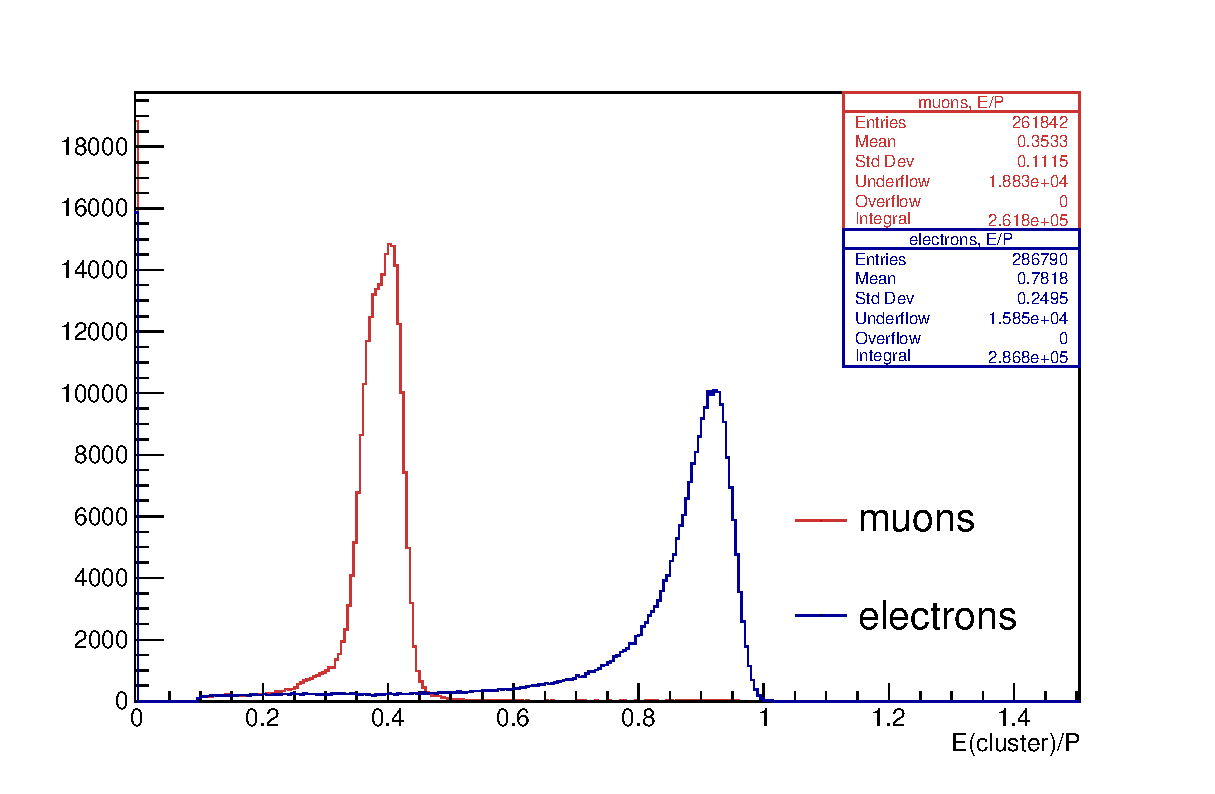
\includegraphics[width=0.65\textwidth]{figures/pdf/figure_00300_pid_emuana_1070_trk_101_ep}
    % }
  };
  \node[anchor=south west,inner sep=0] at (7.5,0.) {
    % \node[shift={(0 cm,0.cm)},inner sep=0,rotate={90}] at (0,0) {}
    % \makebox[\textwidth][c] {
    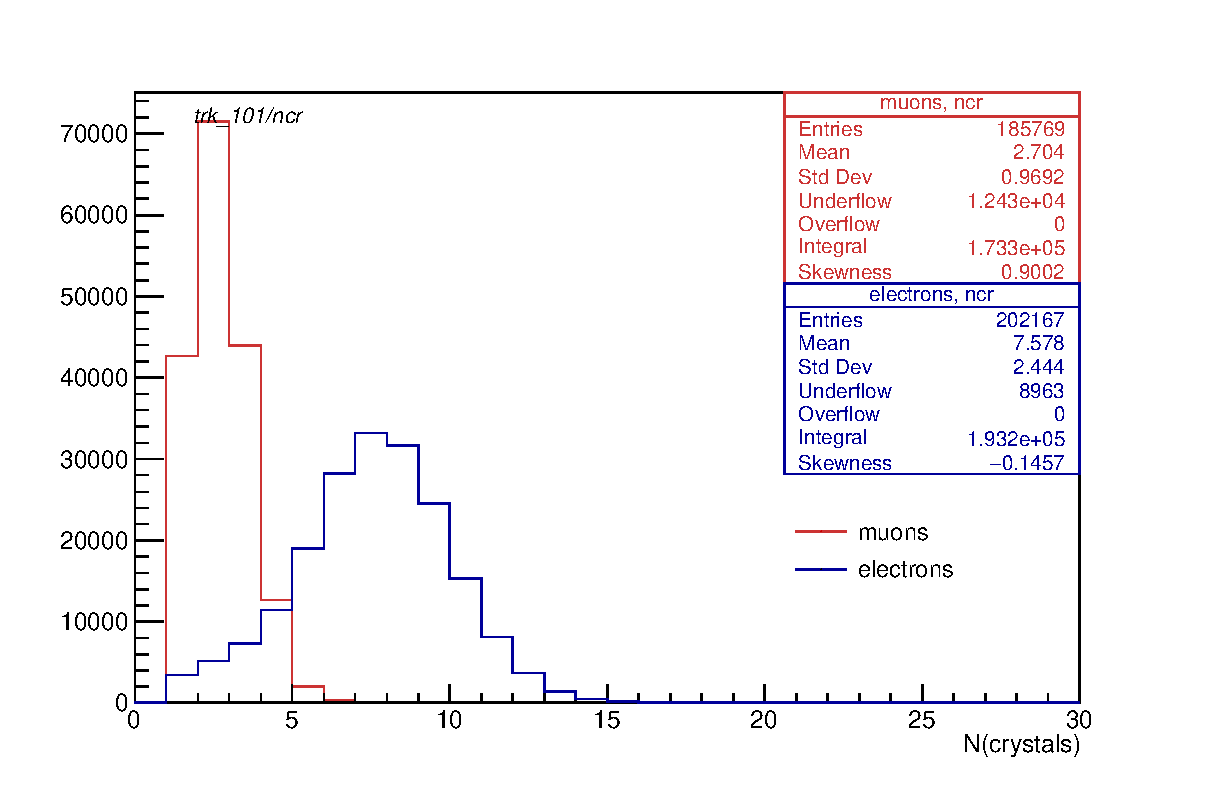
\includegraphics[width=0.65\textwidth]{figures/pdf/figure_00301_pid_emuana_1070_trk_101_ncr}
    % }
  };
  \node[anchor=south west,inner sep=0] at (-1,-5.5) {
    % \node[shift={(0 cm,0.cm)},inner sep=0,rotate={90}] at (0,0) {}
    % \makebox[\textwidth][c] {
    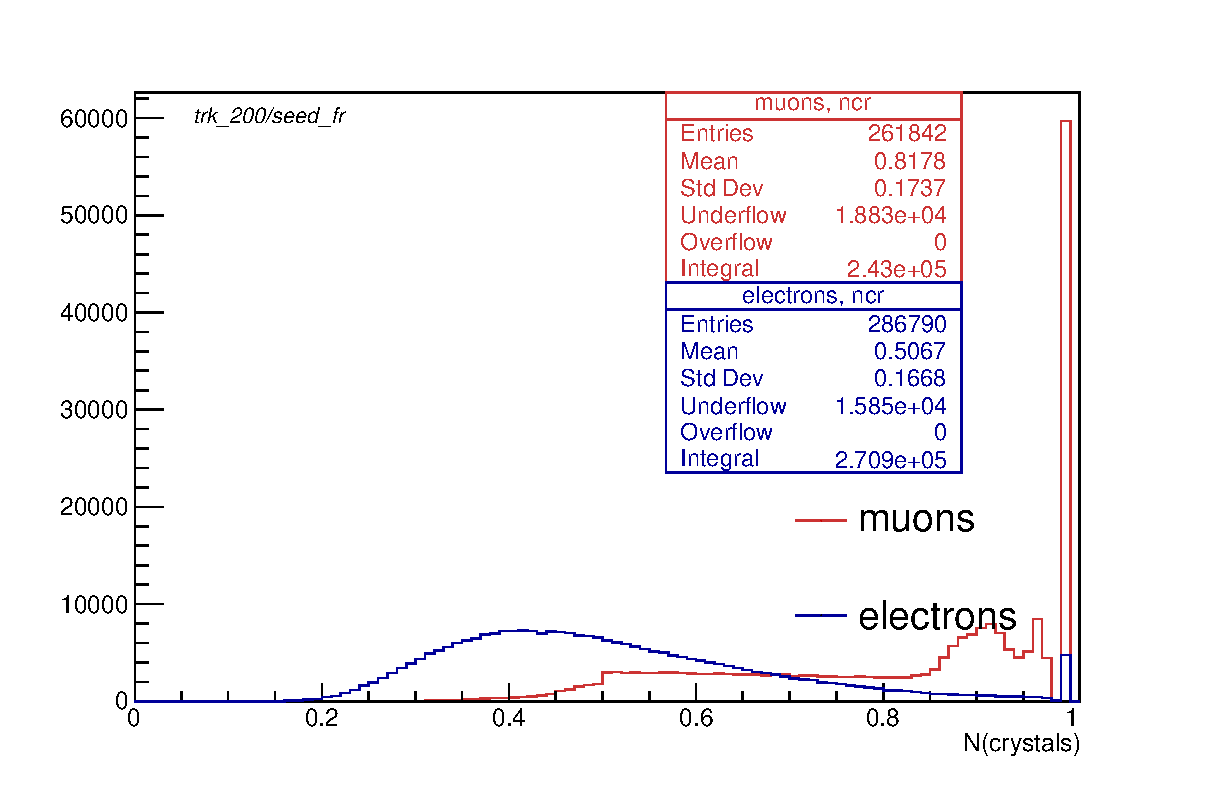
\includegraphics[width=0.65\textwidth]{figures/pdf/figure_00302_pid_emuana_1070_trk_101_seed_fr}
    % }
  };
  \node[anchor=south west,inner sep=0] at (7.5,-5.5) {
    % \node[shift={(0 cm,0.cm)},inner sep=0,rotate={90}] at (0,0) {}
    % \makebox[\textwidth][c] {
    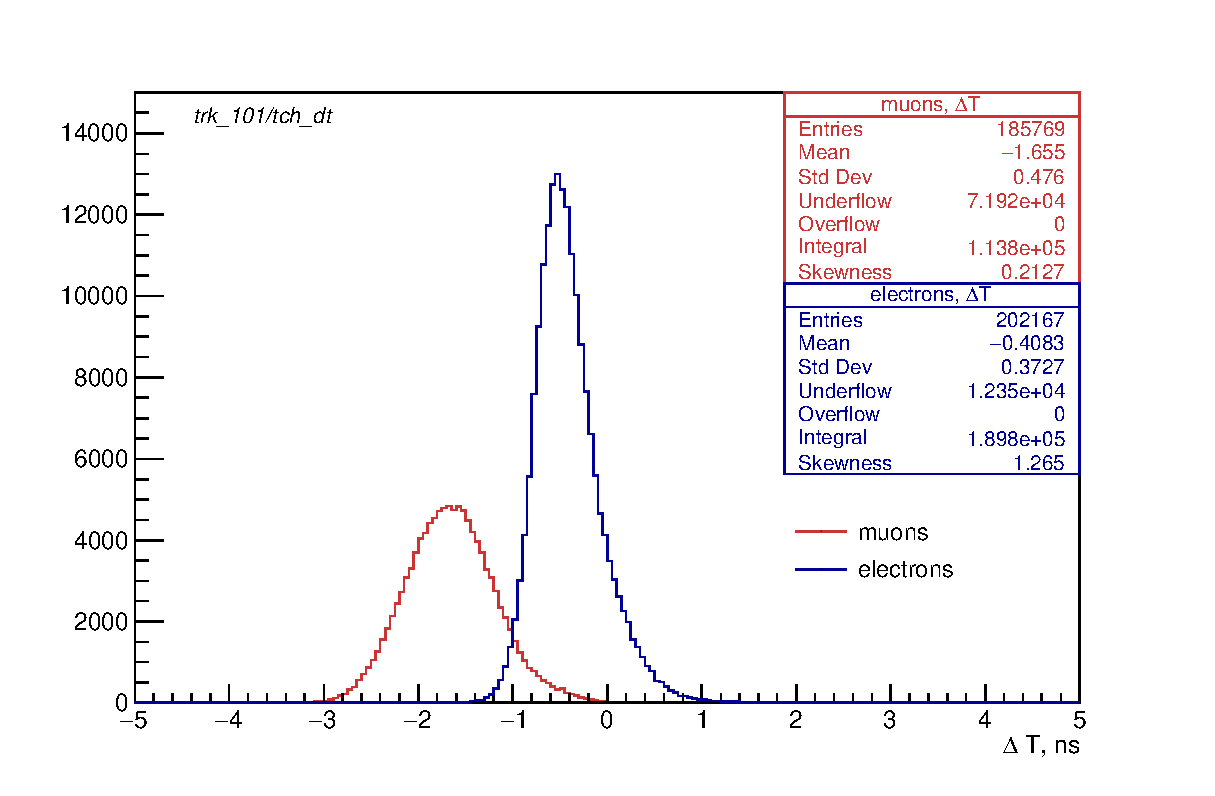
\includegraphics[width=0.65\textwidth]{figures/pdf/figure_00303_pid_emuana_1070_trk_101_tch_dt}
    % }
  };
  \node[anchor=south west,inner sep=0] at (-1,-11.) {
    % \node[shift={(0 cm,0.cm)},inner sep=0,rotate={90}] at (0,0) {}
    % \makebox[\textwidth][c] {
    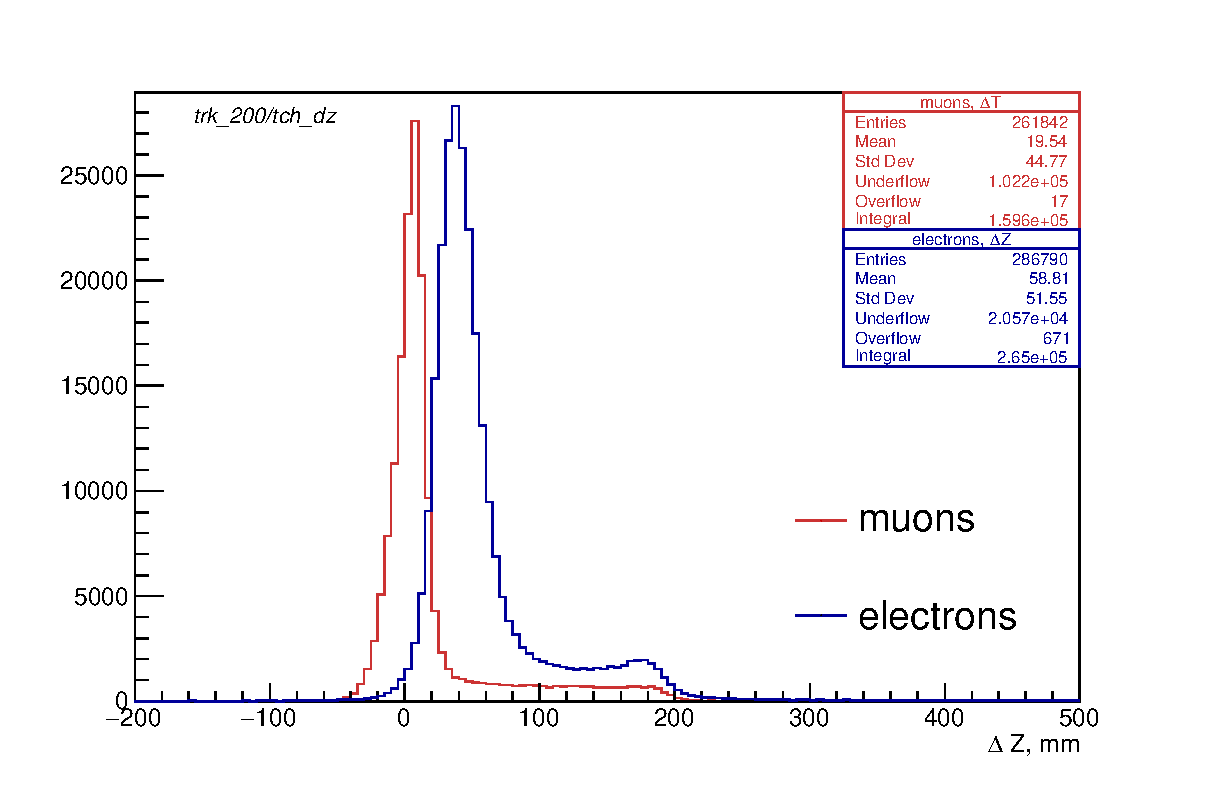
\includegraphics[width=0.65\textwidth]{figures/pdf/figure_00304_pid_emuana_1070_trk_101_tch_dz}
    % }
  };
  \node[anchor=south west,inner sep=0] at (7.5,-11.) {
    % \node[shift={(0 cm,0.cm)},inner sep=0,rotate={90}] at (0,0) {}
    % \makebox[\textwidth][c] {
    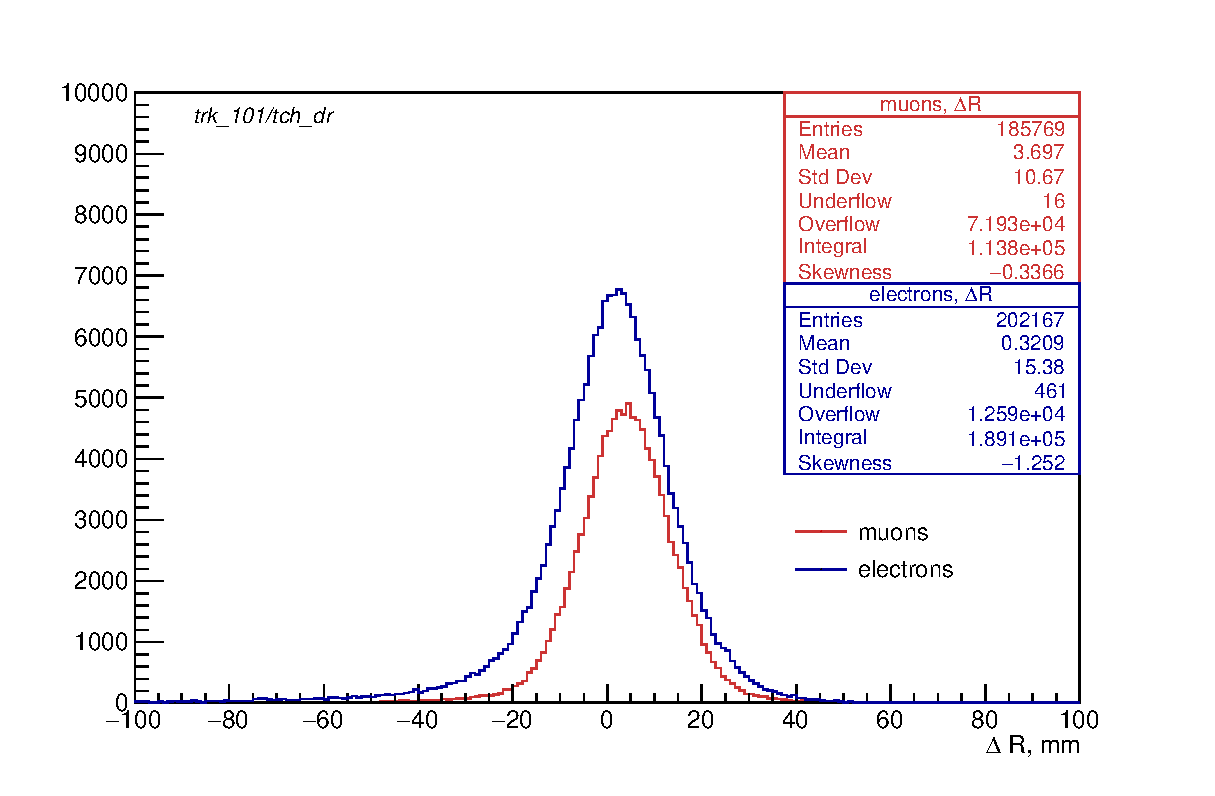
\includegraphics[width=0.65\textwidth]{figures/pdf/figure_00305_pid_emuana_1070_trk_101_tch_dr}
    % }
  };
  % \node [text width=6cm, scale=0.8] at (4.5,6.4) {mu2e-18894 by Kevin Lynch and Jim Popp};
\end{tikzpicture}
% \captionof{figure} {
\caption{
  variables used in PID MVA training
}
\end{figure}

5000 electron and 5000 muon tracks have been used for trainign

Training preselection cuts:

\begin{itemize}
\item 
  reject muon decays in flight: require muon Zmax > 10000,
\item 
  reconstructed track passed electron track selection
\item 
  an event has a reconstructed cluster 
\item 
  $\Delta T > -100$ : some events with reconstructed tracks and clusters had $\Delta T$ undefined
\end{itemize}

\begin{figure}
  \label{fig:pid_training_2}
  \begin{tikzpicture}
    \node[anchor=south west,inner sep=0] at (-1,0.) {
      % \node[shift={(0 cm,0.cm)},inner sep=0,rotate={90}] at (0,0) {}
      % \makebox[\textwidth][c] {
      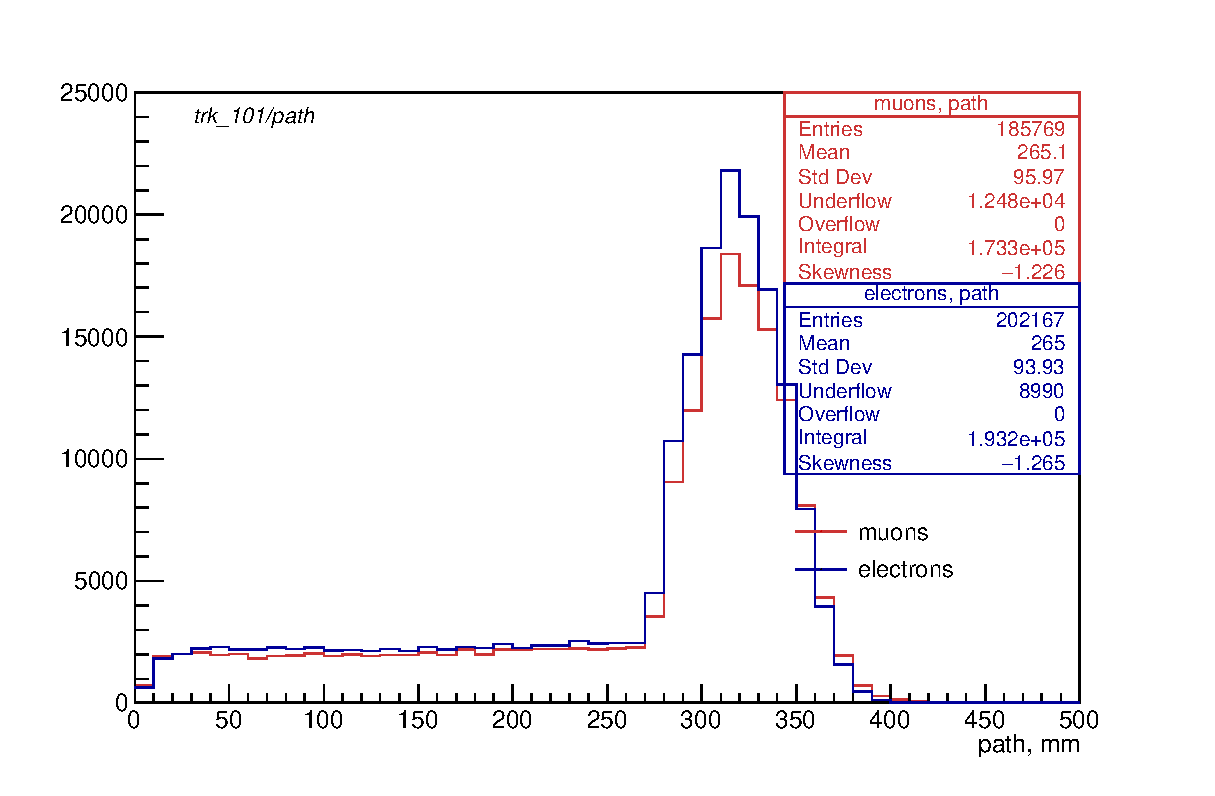
\includegraphics[width=0.65\textwidth]{figures/pdf/figure_00306_pid_emuana_1070_trk_101_path}
      % }
    };
    % \node [text width=6cm, scale=0.8] at (4.5,6.4) {mu2e-18894 by Kevin Lynch and Jim Popp};
  \end{tikzpicture}
  % \captionof{figure} {
  \caption{
    variables used in PID MVA training: particle path in the disk
  }
\end{figure}


training plots :

\begin{figure}
  \label{fig:pid_training_2}
  \begin{tikzpicture}
    \node[anchor=south west,inner sep=0] at (-2,0.) {
      % \node[shift={(0 cm,0.cm)},inner sep=0,rotate={90}] at (0,0) {}
      % \makebox[\textwidth][c] {
      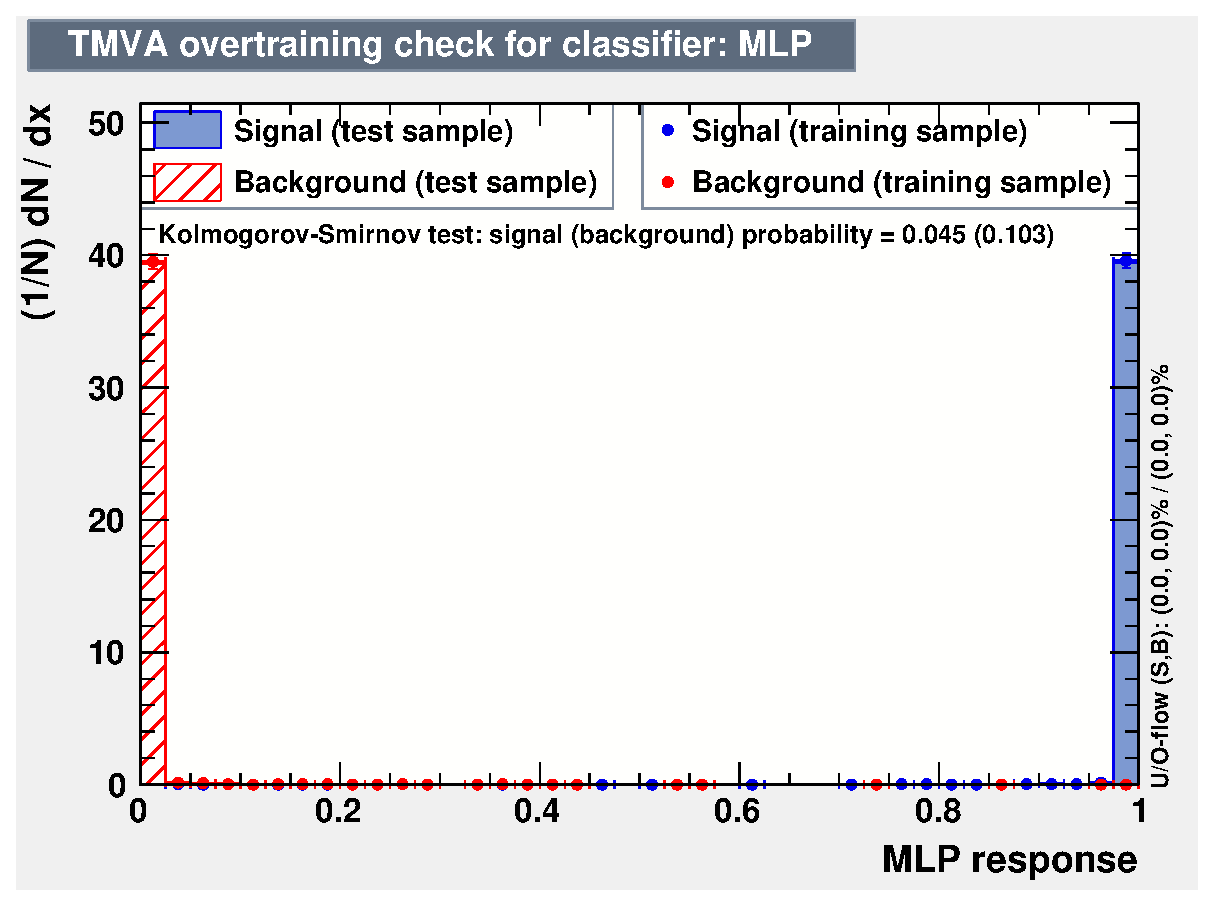
\includegraphics[width=0.60\textwidth]{figures/pdf/pid_mva_overtrain_mlp}
      % }
    };
    \node[anchor=south west,inner sep=0] at (7.5,0.) {
      % \node[shift={(0 cm,0.cm)},inner sep=0,rotate={90}] at (0,0) {}
      % \makebox[\textwidth][c] {
      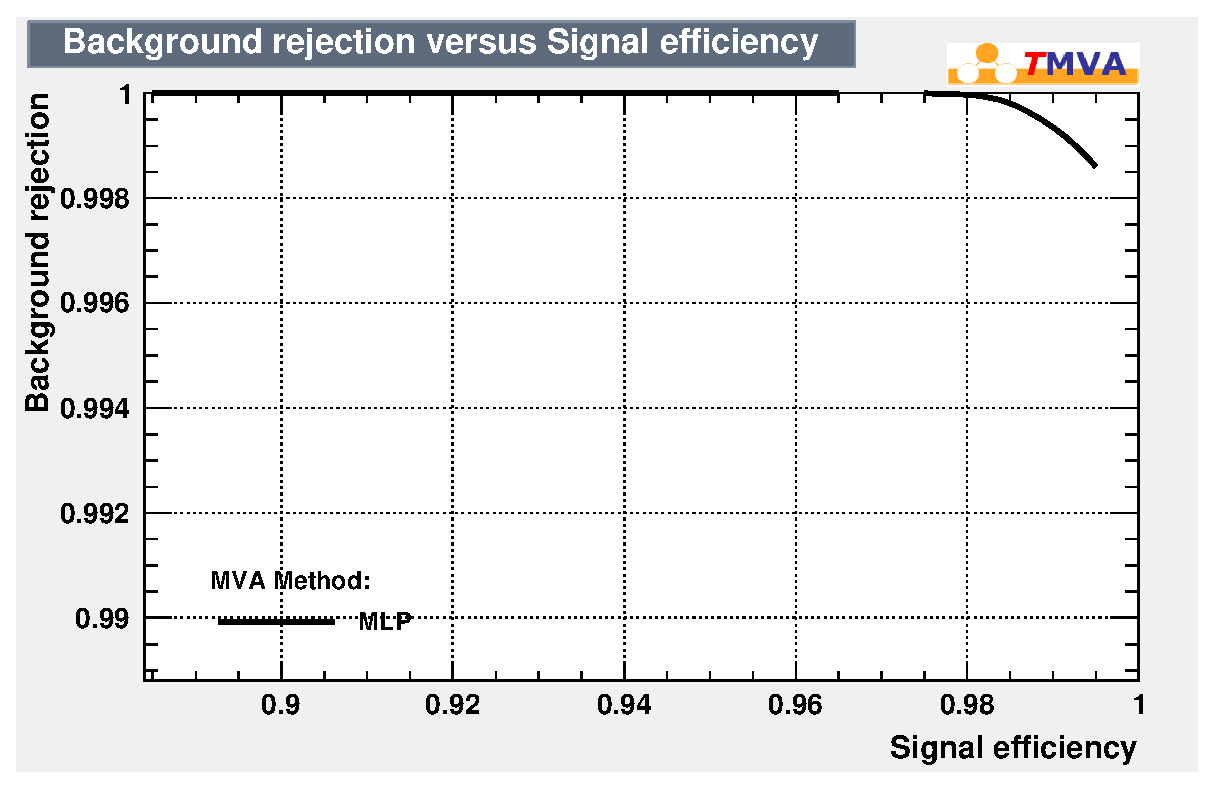
\includegraphics[width=0.60\textwidth]{figures/pdf/pid_mva_rejection_mlp}
      % }
    };
    % \node [text width=6cm, scale=0.8] at (4.5,6.4) {mu2e-18894 by Kevin Lynch and Jim Popp};
  \end{tikzpicture}
  % \captionof{figure} {
  \caption{
    output of the PID ANN training: overtraining check on the left and efficiency vs rejection 
    on the right
  }
\end{figure}



\begin{figure}
  \label{fig:pid_training_2}
  \begin{tikzpicture}
    \node[anchor=south west,inner sep=0] at (0,0.) {
      % \node[shift={(0 cm,0.cm)},inner sep=0,rotate={90}] at (0,0) {}
      \makebox[\textwidth][c] {
        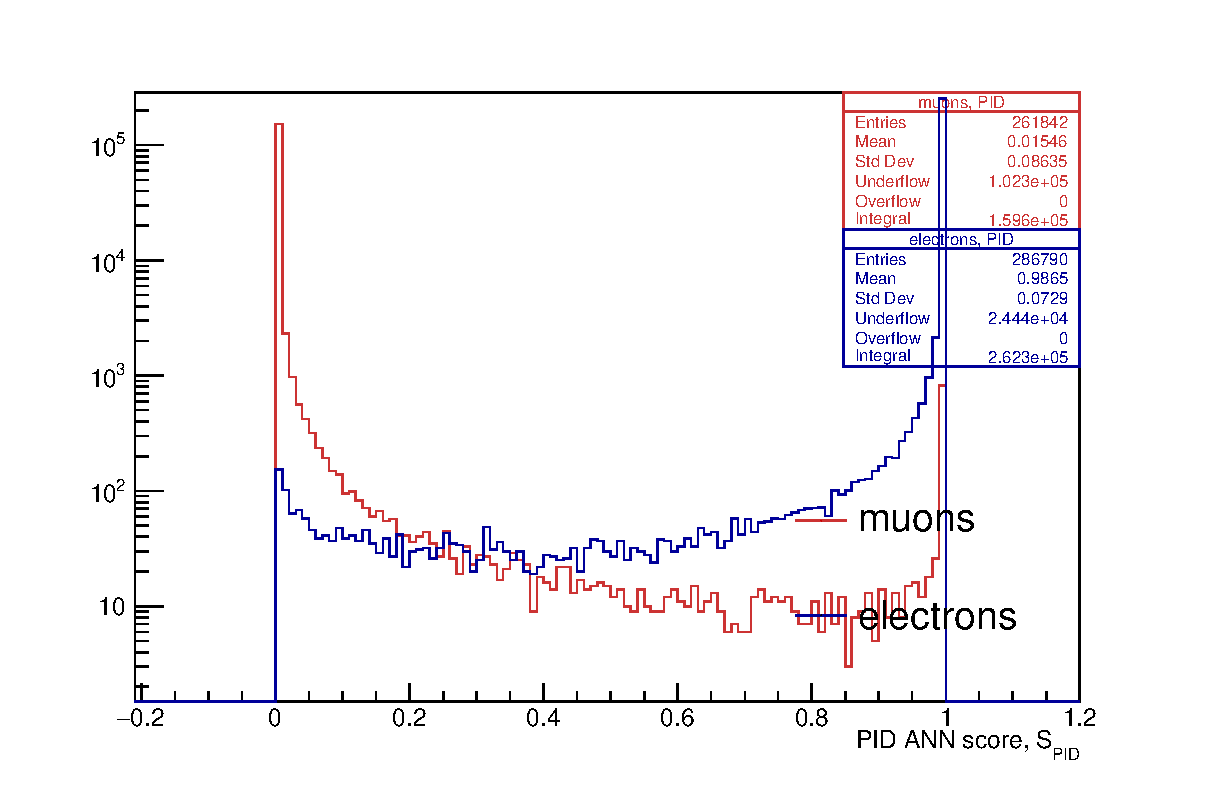
\includegraphics[width=1.0\textwidth]{figures/pdf/figure_00307_pid_emuana_1070_trk_101_pidmvaout}
      }
    };
    % \node [text width=6cm, scale=0.8] at (4.5,6.4) {mu2e-18894 by Kevin Lynch and Jim Popp};
  \end{tikzpicture}
  % \captionof{figure} {
  \caption{
    Distribution in the PID ANN score for electron and muon samples, samples include events used for training,
    5000 events each. A spike in muon PID at 1  - muon decays in flight. \\ 
    {\color{red} \bf Origin of the plotted underflow bin to be investigated}
  }
\end{figure}


PID preselection cuts (ele00s61b0), for reference:

\begin{table}[h!]
  \begin{center}
    \caption{Final Track quality selection}
    \label{tab:table1}
    \begin{tabular}{l|c|c} % <-- Changed to S here.
      \textbf{Cut}                    & \textbf{N events after } & \textbf{Efficiency }\\
      \hline
      total number of tracks          & 343530           &            \\
      \hline
      track passes the selection cuts & 202167           &   0.588    \\
      cluster $E > 10 MeV$            & 193204           &   0.956    \\
      $P > 100$                       & 191012           &   0.989    \\
      $|DR| < 100$ mm                 & 178866           &   {\color{red} \bf 0.936}    \\
      $|DT| < 10$ ns                  & 178866           &   1.0      \\
      $-50 < dz < 250$                & 176619           &   0.987    \\
      $ E/P < 1.2$                    & 176619           &   1.0      \\
      $PID >0.5$                      & 175310           &   0.993    \\
    \end{tabular}
  \end{center}
  \caption{
    PID preselection cuts (ele00s61b0) and efficiency for {\bf ele00s61b0} electrons 
  }
\end{table}

About 6.5\% of all events with tracks and clusters don't have a good track fit, are rejected.
this needs to be investigated.

for electron events with the reconstructed track momentum $P > 100$ MeV/c, passing the preselections, 
the PID efficiency is 0.993


%%%%%%%%%%%%%%%%%%%%%%%%%%%%%%%%%%%%%%%%%%%%%%%%%%%%%%%%%%%%%%%%%%%%%%%%%%%%%%
\newpage
Efficiency for muon events passing the same preselections: 

\begin{itemize}
\item
  $P > 100$                       : 109004
\item 
  $PID >0.5$                      :    799
\end{itemize}

which is about 0.8\%.

Contributing to muon mis-identification are decays of stopped muons with in the calorimeter, early part of the exponential, 
in which the electron energy is counted as the part of the cluster energy

% -*- mode:latex; mode:flyspell -*-


\section{To be investigated} 


\begin{itemize}
\item 
  timing systematics in the track cluster matching
\item 
  events with |TCH\_DR|< 100 and no associated clusters E/P < 0? - but in extrapolation ?
\item
  section \ref{sec:mumep_channel_pid} : spike in the PID score distributions
\item
  section \ref{sec:electrons_failing_pid} : electrons with large value of $R_{max}$
\item
  section \ref{sec:electrons_failing_pid} : electrons with $\Delta{T} < 1.5$ ns
\end{itemize}


\bibliographystyle{unsrtnat}
\bibliography{mu2e_internal_notes,clfv,dio,radiative_muon_capture}
%% \printbibliography
\end{document}


% ------------------------------------------------------------------------------
% templates
% ------------------------------------------------------------------------------
% Table ~\ref{table:summary} gives summary the numbers used in this study.
% 
% \hspace{-0.1in}
% \begin{table}[htbp]
%   \label{table:summary}
%   \begin{center} 
%     {\renewcommand{\arraystretch}{1.0}   % change 1.0 to 1.1 to increase the spacing between the table lines
%       \begin{tabular}{|c|c|c|c|}
%         \hline
%                             & default TS geometry & misaligned TS geometry   &  Ratio(default/misaligned)    \\ 
%         \hline
%         $N_{POT}$            &  $4.96 \cdot 10^6$  &    $5.00 \cdot 10^6$      &   0.992   \\ 
%         $N_{\mu}^{TS3u}$      &  65648              &     61354                 &   1.070   \\ 
%         $N_{\mu}^{TS5}$       &  28517              &     27351                 &   1.043   \\ 
%         $N_{\mu}^{ST}$        &  8868               &      8396                 &   1.056   \\ 
%         $N_{\mu}^{ST}/N_{POT}$ &  $1.79 \pm 0.02$    &    $1.68 \pm 0.02$        &   $1.065 \pm 0.03$        \\ 
%         \hline
%       \end{tabular}
%     }
%   \end{center}
%   \caption{
%     Muons rates at different points of the Mu2e beamline and stopping muon rates for nominal and 
%     misaligned TS geometries
%   }
%   % \vspace{0.5in}
% \end{table}
